\PassOptionsToPackage{dvipsnames,svgnames,table}{xcolor}
\documentclass[11pt]{article}
\usepackage[a4paper,margin=22mm]{geometry}
\usepackage[no-math]{fontspec}
\setmainfont{DejaVu Serif}
\usepackage{amsmath,amssymb,amsthm,mathtools,graphicx,xcolor,hyperref,xurl,xspace,ifthen,enumerate}
\usepackage[shortlabels]{enumitem}
\setlength{\emergencystretch}{4em}
\AtBeginDocument{\special{pdf:mapline pzdr Dingbats <uzdr.pfb}}
\SetMathAlphabet{\mathbf}{normal}{OT1}{cmr}{bx}{n}
\SetMathAlphabet{\mathbf}{bold}{OT1}{cmr}{bx}{n}
\usepackage{thmtools}
\usepackage[capitalize]{cleveref}
\newtheorem{theo}{Theorem}[section]
\newtheorem{lemm}[theo]{Lemma}
\newtheorem{thm}[theo]{Theorem}
\newtheorem{proposition}[theo]{Proposition}
\newtheorem{corollary}[theo]{Corollary}
\newtheorem{definition}[theo]{Definition}
\newtheorem{theorem}[theo]{Theorem}
\newtheorem*{remas*}{Remarks}
\newtheorem{remas}[theo]{Remarks}
\newtheorem*{exam*}{Example}
\newtheorem{ques}[theo]{Question}
\providecommand{\og}{«\nobreakspace}
\providecommand{\fg}{\nobreakspace»}
\newtheorem{lem}[theo]{Lemma}
\newtheorem{lemma}[theo]{Lemma}
\newtheorem{prop}[theo]{Proposition}
\newtheorem{coro}[theo]{Corollary}
\newtheorem{corol}[theo]{Corollary}
\newtheorem*{conj*}{Conjecture}
\newtheorem{conj}[theo]{Conjecture}
\newtheorem{conjecture}[theo]{Conjecture}
\newtheorem{Proposition}[theo]{Proposition}
\newtheorem{theoreme}[theo]{Theorem}
\theoremstyle{definition}
\newtheorem{defi}[theo]{Definition}
\newtheorem{exam}[theo]{Example}
\newtheorem{exem}[theo]{Example}
\newtheorem{remark}[theo]{Remark}
\newtheorem{example}[theo]{Example}
\newtheorem{exams}[theo]{Examples}
\newtheorem{rema}[theo]{Remark}
\newtheorem{nota}[theo]{Notation}
\newtheorem{notation}[theo]{Notation}
\newtheorem*{notas}{Notations}
\newtheorem{result}[theo]{Result}
\newtheorem{question}[theo]{Question}
\newtheorem{prob}[theo]{Problem}
\newtheorem*{rema*}{Remark}
\newtheorem*{defi*}{Definition}
\newtheorem*{theo*}{Theorem}
\newtheorem*{lemm*}{Lemma}
\newtheorem*{prop*}{Proposition}
\newcommand{\enoncename}{}
\newtheorem{corpusenonce}[theo]{\enoncename}
\newenvironment{enonce}[2][]{\renewcommand{\enoncename}{#2}\begin{corpusenonce}}{\end{corpusenonce}}
\newenvironment{enonce*}[2][]{\par\medskip\noindent\textbf{#2.}\itshape}{\par\medskip}
\newenvironment{proofc}[1][\proofname]{\begin{proof}[#1]}{\end{proof}}
\newcommand{\Mc}{\mathcal{M}}
\newcommand{\pointir}{.\ ---\ }
\newcommand{\equalenv}[2]{\expandafter\let\csname#1\expandafter\endcsname\csname#2\endcsname\expandafter\let\csname end#1\expandafter\endcsname\csname end#2\endcsname}
\providecommand{\diagbox}[3][]{\begin{tikzpicture}[x=1em,y=1em,baseline=(current bounding box.center)]\useasboundingbox(0,0) rectangle(3,1.4);\draw(0,1.4)--(3,0);\node at(.5,.3){#2};\node at(2.5,1.1){#3};\end{tikzpicture}}
\providecommand{\eg}{e.g.\ }
\providecommand{\ie}{i.e.\ }
\providecommand{\cf}{cf.\ }
\providecommand{\longthanks}[1]{\par\smallskip\noindent #1\par\smallskip}
\providecommand{\qbinom}[2]{\genfrac{[}{]}{0pt}{}{#1}{#2}}

\providecommand{\mathof}[1]{\mathrm{#1}}

\numberwithin{equation}{section}


\def\endappendix{}


\usepackage{amsmath,amssymb,amsthm,amsfonts}
\usepackage{mathtools}

\usepackage{tikz,graphicx,color}
\usepackage{tikz-cd}
\usepackage{tikz-3dplot}
\usetikzlibrary{calc}
\usetikzlibrary{arrows}
\usetikzlibrary{shapes}
\usetikzlibrary{patterns}
\usetikzlibrary{positioning}
\usetikzlibrary{arrows.meta}
\usetikzlibrary{knots}
\usetikzlibrary{decorations.markings}
\usepackage{epstopdf}

\usepackage[arrow]{xy}

\usepackage{subfig}
\usepackage{arcs}
\usepackage{xcolor}
\usepackage{tabu}
\usepackage{booktabs}

% Unused soul import omitted; no soul text-markup commands occur in retained native body.

\usepackage{letltxmacro}
\usepackage{thmtools,etoolbox}
\usepackage{nameref,hyperref}
\usepackage[capitalize]{cleveref}

\usepackage{tikz-cd}
\usepackage{xspace}

\usepackage{bm}

\newcommand\Acal{\mathcal{A}}\newcommand\Bcal{\mathcal{B}}\newcommand\Ccal{\mathcal{C}}\newcommand\Dcal{\mathcal{D}}\newcommand\Ecal{\mathcal{E}}\newcommand\Fcal{\mathcal{F}}\newcommand\Gcal{\mathcal{G}}\newcommand\Hcal{\mathcal{H}}\newcommand\Ical{\mathcal{I}}\newcommand\Jcal{\mathcal{J}}\newcommand\Kcal{\mathcal{K}}\newcommand\Lcal{\mathcal{L}}\newcommand\Mcal{\mathcal{M}}\newcommand\Ncal{\mathcal{N}}\newcommand\Ocal{\mathcal{O}}\newcommand\Pcal{\mathcal{P}}\newcommand\Qcal{\mathcal{Q}}\newcommand\Rcal{\mathcal{R}}\newcommand\Scal{\mathcal{S}}\newcommand\Tcal{\mathcal{T}}\newcommand\Ucal{\mathcal{U}}\newcommand\Vcal{\mathcal{V}}\newcommand\Wcal{\mathcal{W}}\newcommand\Xcal{\mathcal{X}}\newcommand\Ycal{\mathcal{Y}}\newcommand\Zcal{\mathcal{Z}}

\newcommand\abf{\mathbf{a}}\newcommand\bbf{\mathbf{b}}\newcommand\cbf{\mathbf{c}}\newcommand\dbf{\mathbf{d}}\newcommand\ebf{\mathbf{e}}\newcommand\fbf{\mathbf{f}}\newcommand\gbf{\mathbf{g}}\newcommand\hbf{\mathbf{h}}\newcommand\ibf{\mathbf{i}}\newcommand\jbf{\mathbf{j}}\newcommand\kbf{\mathbf{k}}\newcommand\lbf{\mathbf{l}}\newcommand\mbf{\mathbf{m}}\newcommand\nbf{\mathbf{n}}\newcommand\obf{\mathbf{o}}\newcommand\pbf{\mathbf{p}}\newcommand\qbf{\mathbf{q}}\newcommand\rbf{\mathbf{r}}\newcommand\sbf{\mathbf{s}}\newcommand\tbf{\mathbf{t}}\newcommand\ubf{\mathbf{u}}\newcommand\vbf{\mathbf{v}}\newcommand\wbf{\mathbf{w}}\newcommand\xbf{\mathbf{x}}\newcommand\ybf{\mathbf{y}}\newcommand\zbf{\mathbf{z}}

\newcommand\C{\mathbb{C}}
\newcommand\R{\mathbb{R}}
\newcommand\N{\mathbb{N}}
\newcommand\Z{\mathbb{Z}}
\newcommand\Q{\mathbb{Q}}

\newcommand\Ahat{\hat{A}} 
\newcommand\ipar{{(i)}}
\newcommand\parr[1]{{({#1})}}


\newcommand\m{{\mu}}
\newcommand\lm{{\l/\m}}

\newcommand\Id{\operatorname{Id}}
\newcommand\Vol{\operatorname{Vol}}
\newcommand\diag{{ \operatorname{diag}}}
\newcommand\rank{{ \operatorname{rank}}}
\newcommand\rk{{\mathrm{rank}}}
\newcommand\cork{ \operatorname{corank}}
\newcommand\corank{ \operatorname{corank}}
\newcommand\codim{ \operatorname{codim}}
\newcommand\op{{ \operatorname{op}}}
\newcommand\sh{{ \operatorname{sh}}}
\newcommand\Conv{ \operatorname{Conv}}
\newcommand\Span{ \operatorname{Span}}
\newcommand\proj{ \operatorname{proj}}
\newcommand\sgn{ \operatorname{sgn}}
\newcommand\wt{\operatorname{wt}}
\newcommand\inv{\operatorname{inv}}
\newcommand\Int{\operatorname{int}}
\newcommand\Cone{\operatorname{Cone}}

\newcommand\GL{\operatorname{GL}}
\newcommand\SL{\operatorname{SL}}
\newcommand\Mat{\operatorname{Mat}}
\newcommand\Gr{\operatorname{Gr}}
\newcommand\Grtnn{\Gr_{\ge 0}}
\newcommand\Grtp{\Gr_{>0}}
\newcommand\alt{\operatorname{alt}}
\newcommand\Mattp{\operatorname{Mat}_{>0}}
\newcommand\Mattnn{\operatorname{Mat}_{\ge0}}


\newcommand\Bound{{\rm Bound}}

\newcommand\af{{\rm af}}
\newcommand\Inv{{\rm Inv}}

\newcommand\id{{\operatorname{id}}}

\newcommand\xs{\operatorname{xs}}
\newcommand\ys{\operatorname{ys^{-1}}}
\newcommand\bs{\backslash}
\newcommand\oPi{\accentset{\circ}{\Pi}}
\newcommand\bt{{\mathbf{t}}}
\newcommand\bw{{\mathbf{w}}}
\newcommand\bv{{\mathbf{v}}}
\newcommand\bu{{\mathbf{u}}}
\newcommand\ba{{\mathbf{a}}}
\newcommand\bb{{\mathbf{b}}}
\newcommand\bc{{\mathbf{c}}}
\newcommand\geqJ{\succeq}
\newcommand\gessJ{\succ}

\newcommand\bx{{\bm{x}}}
\newcommand\by{{\bm{y}}}
\newcommand\bi{{\mathbf{i}}}
\newcommand\bj{{\mathbf{j}}}




\newcommand\Deltamp{\Delta^\mp}
\newcommand\Deltapm{\Delta^\pm}


\newcommand\RedMR{\operatorname{Red}}
\newcommand\Red{\operatorname{Red}}
\newcommand\weightL{Y(T)}
\newcommand\rootL{Q_\Phi}
\newcommand\Qkls{Q_P(W,W_J)}


\newcommand\chr{\operatorname{char}}

\let \oldlabel \label
\let\oldref\ref
\let\oldcref\cref





\newcommand\B{{\mathcal B}}
\newcommand\G{\Gcal}
\newcommand\Caff{{\mathcal{C}}}
\newcommand\GCMaff{\tilde{A}}

\newcommand\Phiaff{\Delta}
\newcommand\re{\operatorname{re}}
\newcommand\im{\operatorname{im}}
\newcommand\Phire{\Phiaff_{\re}}
\newcommand\Phiim{\Phiaff_{\im}}

\newcommand\FPS{{\mathcal{A}}}
\newcommand\CRL{{\rootL^\vee}}
\newcommand\minn{{\operatorname{min}}}
\newcommand\Cast{\C^\ast}

\newcommand\tauk{\tau_k}
\newcommand\leqop{\leq^\op}
\newcommand{\Povar}{\mathring{\Pi}}

\newcommand\Boundkn{\operatorname{Bound}(k,\n)}


\newcommand\BAcomb{\psi}
\newcommand\BAgeom{\bar\varphi_u}
\newcommand\BAgeo{\varphi_u}

\newcommand\tht{t}





\newcommand\Ng{{N_g}}
\newcommand\strix{t_1(x)}
\newcommand\strixn{t_1(x_n)}
\newcommand\Bcl{\overline{B}}
\newcommand\epsb{\eps_B}


\newcommand\conept{c}

\newcommand\Link{\operatorname{Lk}}

\newcommand\eps{\varepsilon}






\newcommand\Spec{\operatorname{Spec}}

\newcommand\pr{^{\parr{r}}}

\newcommand\om{\omega}
\newcommand\pan{^\parr{n}}

\newcommand*{\smallcap}{{\mathbin{\scalebox{0.5}{\ensuremath{\cap}}}}}

\newcommand\gc{g_\smallcap}
\newcommand\BG{B_-\backslash G}
\newcommand\BGtnn{(B_-\backslash G)_{\geq0}}

\newcommand\GBsf{(G/B_-)(K)}
\newcommand\BGsf{(\BG)(K)}


\newcommand\str{\operatorname{str}}
\newcommand\strd{\operatorname{str}^\ast}

\newcommand\Sn{S_\n}
\newcommand\chiv{\vec\chi_{v}}

\newcommand\chiw{\vec\chi^{\,w}}
\newcommand\chiww{\vec\chi^{\,{\ww}}}

\newcommand\flec{\vec f}
\newcommand\fR{\vec f}


\newcommand\Ztnn{\Z_{\geq0}}


\newcommand\colspan{\operatorname{ColumnSpan}}

\newcommand\Qkn{Q_{k,\n}}
\newcommand\Bkn{\Boundkn}
\newcommand\Skn{S_\n^{(k)}}

\newcommand\perm{\operatorname{perm}}
\newcommand\Lperm{L^{\perm}}
\newcommand\tor{\operatorname{tor}}
\newcommand\Ltor{L^{\tor}}
\newcommand\grid{\operatorname{grid}}
\newcommand\Lgrid{L^{\grid}}
\newcommand\Lgridt{\tilde L^{\grid}}
\newcommand\rich{\operatorname{Rich}}
\newcommand\Lrich{L^{\rich}}
\newcommand\plab{\operatorname{plab}}
\newcommand\Lplab{L^{\plab}}
\newcommand\cox{\operatorname{Cox}}
\newcommand\Lcox{L^{\cox}}

\newcommand\fp{\pi}


\newcommand\pig{\pi_G}

\newcommand\Arg{\operatorname{arg}}

\newcommand\ice{\operatorname{ice}}
\newcommand\QG{Q_G}
\newcommand\Qice{\widetilde{Q}}
\newcommand\QGice{\Qice_G}

\newcommand\BQ{B(Q)}
\newcommand\BQice{\widetilde{B}(\Qice)}
\newcommand\Vice{\widetilde{V}}

\newcommand\AQ{\Acal(Q)}
\newcommand\AQG{\Acal(\QG)}
\newcommand\AQGice{\Acal(\QGice)}
\def\RQ(#1){R(Q;#1)}
\def\RQX#1#2{R(#1;#2)}
\def\RQice(#1){R(\Qice;#1)}
\def\RQG(#1){R(\QG;#1)}
\newcommand\F{\mathbb{F}}

\newcommand\Pio{\Pi^\circ}
\newcommand\HOMP{P}
\newcommand\unknot{
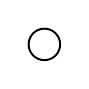
\begin{tikzpicture}[baseline=(ZUZU.base),scale=0.2]\coordinate(ZUZU) at (0,-0.6);
\draw[line width=0.7pt] (0,0) circle (1cm);
  \end{tikzpicture}
}


\newcommand\Top{{\operatorname{top}}}
\def\Ptop_#1(#2){P^\Top(#1;#2)}

\newcommand\fbar{\bar f}
\newcommand\taukn{\tau_{k,\n}}
\newcommand\T{\mathbb{T}}

\newcommand\Cproj{\overline{C}}


\newcommand\fro{\operatorname{fro}}
\newcommand\mut{\operatorname{mut}}
\newcommand\Vfro{V_{\fro}}
\newcommand\Vmut{V_{\mut}}
\newcommand\bip{\operatorname{bip}}
\newcommand\Gbip{G^{\bip}}



\def\Qicefr[#1]{\Qice[#1]}
\newcommand\Bice{\widetilde{B}}
\newcommand\bice{\tilde{B}}
\newcommand\XQice{\Xcal(\Qice)}
\newcommand\XBQice{\Xcal(\BQice)}
\newcommand\AX{\Acal}
\newcommand\AQice{\Acal(\Qice)}
\newcommand\ABQice{\Acal(\BQice)}

\newcommand\chiQ{\chi_Q}
\newcommand\chiQice{\chi_{\Qice}}

\newcommand\Gm{\F^\ast}
\newcommand\Ga{\F}


\newcommand\Aut{\operatorname{Aut}}
\def\QX(#1){Q_{#1}}
\newcommand\disjun{\sqcup}
\newcommand\pmi{\pm I}
\newcommand\pmim{(\pmi)^m}

\newcommand\pmn{\pm I}
\newcommand\pmnm{(\pmn)^m} 
\newcommand\DRW{(\pmn)^m} 

\newcommand\Gbw{G(\bw)}
\def\GX(#1){G(#1)}

\newcommand\rev{\operatorname{rev}}


\newcommand\rowspan{\operatorname{RowSpan}}

\def\figref#1(#2){Figure~\hyperref[#1]{\ref*{#1}(#2)}}

\newcommand\conn{\operatorname{c}}
\newcommand\ncyc{\conn}

\newcommand\n{N}
\newcommand\qq{q^{\frac12}}
\newcommand\qqi{q^{-\frac12}}

\newcommand\disk{\mathbf{D}}

\newcommand\Lrichp{L}

\newcommand\projt{p_{\T}}
\def\projtx#1{\overline{#1}}

\newcommand\Louise{locally acyclic\xspace}
\newcommand\Louiseleaf{recurrent leaf\xspace} 


\newcommand\degtop{\deg^{\Top}}
\newcommand\tI{{\tilde I}}
\newcommand\pmtI{\pm\tI}
\def\linkurl#1{\textup{\texttt{\href{http://katlas.org/wiki/#1}{#1}}}}
\newcommand\comma{} 

\newcommand\Btilde{$\tilde{\text{B}}$}



\def\hopflink{
\scalebox{0.3}{
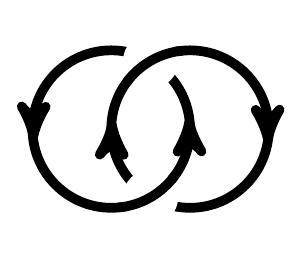
\begin{tikzpicture}[baseline=(ZUZU.base)]\coordinate(ZUZU) at (0,-0.8);
\draw[line width=3.5pt, white,
    decoration={markings,mark=at position 0 with {\arrow[scale=1,black]{stealth'}}},
    decoration={markings,mark=at position 1 with {\arrow[scale=1,black]{stealth'}}},
    postaction={decorate}] (-0.99,-0.15)--(-1,-1)--(1,-1)--(0.99,0.15);
\draw[line width=3.5pt, white,
    decoration={markings,mark=at position 0.01 with {\arrow[scale=1,black]{stealth'}}},
    decoration={markings,mark=at position 0.99 with {\arrow[scale=1,black]{stealth'}}},
    postaction={decorate}] (1.99,-0.15)--(2,-1)--(0,-1)--(0.01,0.15);
\begin{knot}[
    clip width=6,
    flip crossing={1},
    ]
    \strand [line width=3.5pt] (0,0) circle (1.0cm);
    \strand [line width=3.5pt] (1,0) circle (1.0cm);
\end{knot}
\end{tikzpicture} 
}
}

\newcommand\pikn{\pi_{k,\n}}
\newcommand\fkn{f_{k,\n}}


\newcommand\pA{^{(1)}}
\newcommand\pB{^{(2)}}
\newcommand\pC{^{(3)}}
\newcommand\pD{^{(4)}}
\newcommand\pE{^{(5)}}
\newcommand\red{-}
\newcommand\Qred{Q^{\red}}
\newcommand\QredG{Q^{\red}_G}
\newcommand\BQredG{B(\QredG)}

\newcommand\E{H}
\newcommand\Tc{{T,c}}

\newcommand\mysq{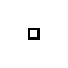
\begin{tikzpicture}
\node[draw=black,line width=1pt, rectangle,scale=0.5,fill=white] (A) at (0,0) {};
\end{tikzpicture}}

\newcommand\tils{\tilde s}


\newcommand\HHH{H\!\!H\!\!H}
\newcommand\HHHC{\HHH_\C}
\newcommand\PGL{\operatorname{PGL}}

\def\mirr#1{#1^\ast}
\newcommand\Divide{\Delta}

\newcommand{\FLY}{HOMFLY\xspace}
\newcommand{\la}{\lambda}
\newcommand{\w}{{\mathbf{w}}}
\newcommand{\pt}{{\rm pt}}
\newcommand{\arxiv}[1]{\href{https://arxiv.org/abs/#1}}



















\begin{document}
\section*{\raggedright 840: Reduced exchange matrices of plabic graphs are torsion-free}
\noindent\textbf{Author:} Galashin, Pavel; Lam, Thomas\par\noindent\textbf{Source:} Plabic links, quivers, and skein relations. Algebraic Combinatorics 7 (2024), publisher version, DOI 10.5802/alco.345. \url{https://alco.centre-mersenne.org/articles/10.5802/alco.345/}
\par\noindent\textbf{License:} CC BY 4.0, \url{https://creativecommons.org/licenses/by/4.0/}. The original publisher PDF cover has the explicit license notice. See the saved source/license records.
\par\noindent\textbf{Editorial material note (not author text):} The selected problem is Proposition6.8: the reduced exchange matrix of every authored plabic graph is integrally torsion-free. The complete author cut-vertex/double-edge reduction and explicit quotient-basis argument for every face case are retained, with exact graph/reduced-quiver definitions and all local move illustrations. The cluster-leaf stratum and HOMFLY identity are separate unselected context. Full local Sections2--7.3 support is retained in source order; unrelated fixed-point sketches, numerical Dynkin examples, the numeric HOMFLY illustration and later conjecture programs are omitted with exact original printed locators. All proof text/formulas and native TikZ remain editable; only bounded original graphical illustrations are assets. The unused Povar helper has no actual retained body uses. No proof or index in a mathematical claim is repaired. All proof text and formulas below are editable author TeX. Mathematical wording, language and proof order are retained. Only the article class, title matter and bibliography presentation are adapted for independent compilation; no proof has been generated or repaired.
\par\noindent\textbf{Editorial difficulty:} H2: The proof reduces plabic graphs through interior leaves, loops and opposite-color double edges, then constructs integral quotient bases in each boundary/interior-face case. The cut-vertex reduction and explicit row relations prove integral torsion-freeness, not just rational matrix rank.
\medskip\hrule\medskip
\noindent\textbf{Author statement, complete proof and local supporting text follow in source order.}
\newtheorem{problem}[theo]{Problem}
%\equalenv{example}{exam}
%\equalenv{notation}{nota}

\crefname{figure}{Figure}{Figures}
\crefname{conjecture}{Conjecture}{Conjectures}
%\equalenv{conjecture}{conj}

\addtotheorempostheadhook[theorem]{\crefalias{theoremlisti}{theorem}}
\addtotheorempostheadhook[lemma]{\crefalias{theoremlisti}{lemma}}
\addtotheorempostheadhook[proposition]{\crefalias{theoremlisti}{proposition}}
\addtotheorempostheadhook[corollary]{\crefalias{theoremlisti}{corollary}}

\setcounter{section}{1}
\section{Main results}
Let $\fp\in\Sn$ be a permutation. For simplicity (cf. Section~4.5), we assume that $\fp$ has no fixed points, i.e.  $\fp(i)\neq i$ for all $i\in[\n]:=\{1,2,\dots,\n\}$. 
 %

\begin{figure}
\begin{tabular}{cccc}
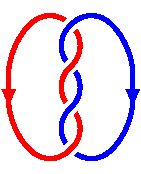
\includegraphics[width=0.13\textwidth]{../assets/840/L4a1.pdf} &
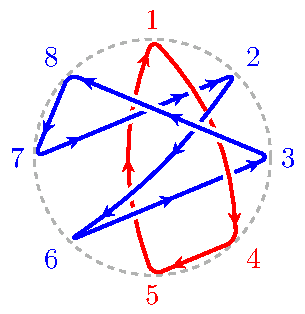
\includegraphics[width=0.27\textwidth]{../assets/840/Lperm.pdf} &
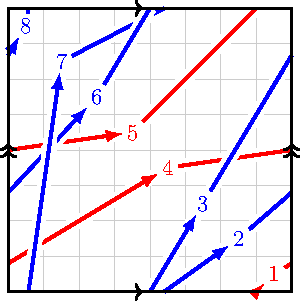
\includegraphics[width=0.24\textwidth]{../assets/840/Ltor.pdf}&
\hspace{0.05in}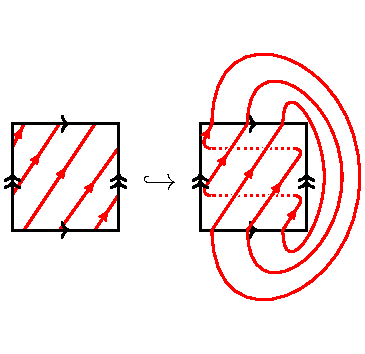
\includegraphics[width=0.25\textwidth]{../assets/840/Ltor_emb.pdf}\\
  (a) \linkurl{L4a1} & (b) $\Lperm_\pi$ & (c) $\Ltor_\pi$ & (d) \hspace{0.05in}$\T\hookrightarrow\R^3$
\end{tabular}
%
%
%
%
%
%
  \caption{\label{fig:L4a1} The links \linkurl{L4a1}$\cong \Lperm_\pi\cong\Ltor_\pi$ for $\pi$ given by~\eqref{eq:intro:fp}.}
\end{figure}


In~\cite{GL_qtcat}, we described a way to associate a \emph{positroid link} $L_\fp$ to such $\fp$. The number of components of $L_\fp$ is given by the number $\ncyc(\fp)$ of cycles of $\fp$. Our running example will be
\begin{equation}\label{eq:intro:fp}
 \fp=\left(\!\!\text{
\begin{tabular}{cccccccc}
\textcolor{red}{$1$} & \textcolor{blue}{$2$} & \textcolor{blue}{$3$} & \textcolor{red}{$4$} & \textcolor{red}{$5$} & \textcolor{blue}{$6$} & \textcolor{blue}{$7$} & \textcolor{blue}{$8$}\\
\textcolor{red}{$4$} & \textcolor{blue}{$6$} & \textcolor{blue}{$8$} & \textcolor{red}{$5$} & \textcolor{red}{$1$} & \textcolor{blue}{$3$} & \textcolor{blue}{$2$} & \textcolor{blue}{$7$}
\end{tabular}
}\!\!\right),
\end{equation}
written in two-line notation, with different colors representing different cycles of $\fp$. We have $\n=8$ and $\ncyc(\fp)=2$. The associated positroid link $L_\fp$ is shown in \figref{fig:L4a1}(a); it appears under the name \linkurl{L4a1} in the Thistlethwaite Link Table~\cite{KAT}. 

\subsection{Positroid links} \label{sec:intro:positroid_links}

Our first result relates several different representations of the link $L_\fp$, confirming the conjectures of~\cite{GL_qtcat,GL_cat_combin}. We start by giving a brief overview of these descriptions; see \cref{sec:positr-comb,sec:positr-link-isot} for full details.

\subsubsection{Permutation link} \label{sec:intro:perm_links}
Draw $\n$ points labeled $1,2,\dots,\n$ on the circle in clockwise order. Draw a line segment connecting $i$ to $\fp(i)$, for each $i\in[\n]:=\{1,2,\dots,\n\}$. If two line segments $[i, \fp(i)]$, $[j,\fp(j)]$ cross for some $i,j\in[\n]$ such that $\fp(i)<\fp(j)$, then the segment $[j,\fp(j)]$ is drawn above $[i, \fp(i)]$; see \figref{fig:L4a1}(b). 
%
 The union of these segments gives rise to a link diagram. We refer to the resulting link as the \emph{permutation link} of $\fp$, denoted $\Lperm_\fp$. Orienting each line segment from $i$ to $\fp(i)$ induces an orientation on $\Lperm_\fp$.


\subsubsection{Toric permutation link}\label{sec:intro:tor_links} Let $\T:=\R^2/\Z^2$ be the torus. Consider its fundamental domain $[0,1]^2$ which we view as a square subdivided into $\n^2$ boxes of size $\frac1\n\times \frac1\n$. We denote by $b_{i,j}$, $1\leq i,j\leq \n$, the box whose upper right corner has coordinates $\frac1\n(i,j)$. For each $i\in[\n]$, place a dot $d_i$ in box $b_{i,\n+1-i}$. Draw an arrow (in $\T$) in the northeast direction from $d_i$ to $d_{\fp(i)}$ for each $i\in[\n]$. When two such arrows cross, the arrow with the higher slope is drawn above the arrow with the lower slope. We obtain a planar diagram of an oriented link $\Ltor_\fp$ drawn on the surface of $\T$; see \figref{fig:L4a1}(c). Any link drawn on $\T$ may be converted into a link in $\R^3$ using the procedure shown in \figref{fig:L4a1}(d). Abusing notation, we denote by $\Ltor_\fp$ the resulting link in $\R^3$.

\begin{remark}
Viewing $\Ltor_\fp$ as drawn on the surface of $\T$ (resp. in a solid torus $S^1\times [0,1]^2$) contains more information---it gives rise to a certain elliptic Hall algebra element~\cite{ScVa,BuSc} (resp. to a symmetric 
%
function~\cite{Turaev}) with deep connections to Khovanov--Rozansky homology. We aim to pursue this direction in an upcoming paper~\cite{GL_EHA}.
\end{remark}
%
%


\begin{figure}
  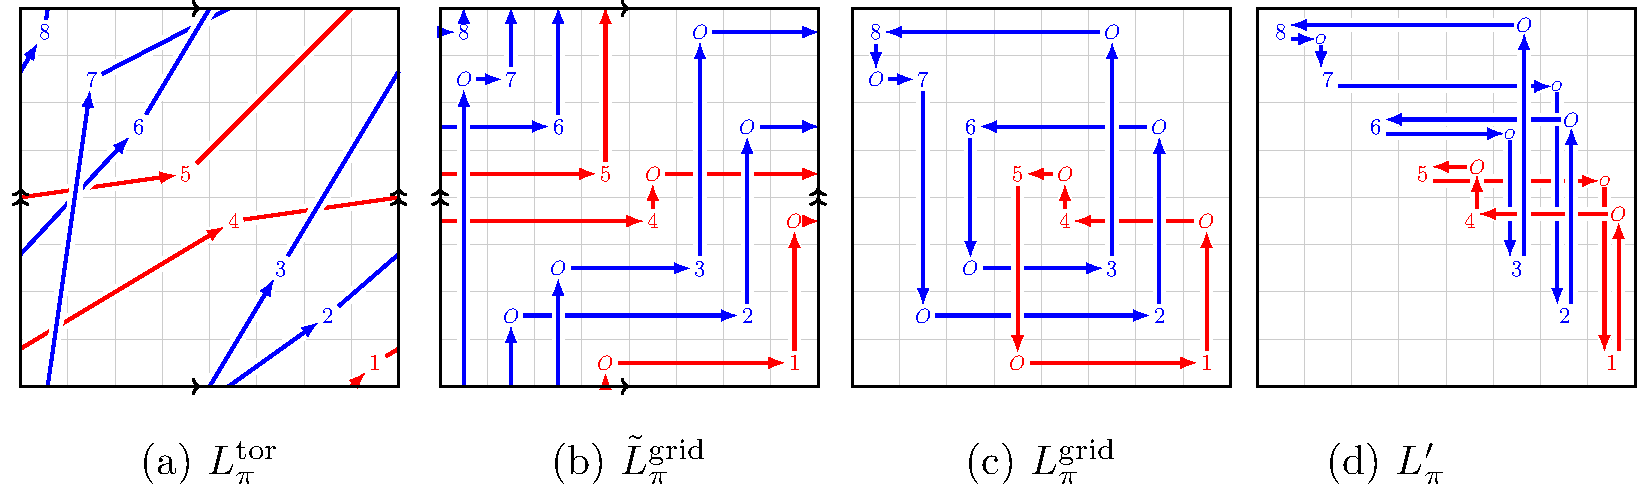
\includegraphics[width=1.0\textwidth]{../assets/840/grid_iso.pdf}
  %
 \caption{\label{fig:grid_iso} Toric grid links; see \cref{rmk:grid} and \cref{sec:perm-to-toric}.}
\end{figure}


\begin{remark}\label{rmk:grid}
We may also view $\Ltor_\fp$ as coming from a \emph{grid diagram} (see e.g.~\cite{OSS}). The grid diagram of $\fp$ is obtained by placing an $X$ in box $b_{i,\n+1-i}$ and an $O$ in box $b_{i,\n+1-\fp(i)}$ for each $i\in[\n]$. We then connect the $X$'s and the $O$'s by horizontal and vertical segments, always drawing the vertical segments above the horizontal ones. More precisely, to a given grid diagram, we can associate two links. First, a \emph{toric grid link} $\Lgridt_\pi$, drawn on the surface of $\T$, is obtained by drawing a horizontal arrow from $O$ to $X$ pointing right in each row, and a vertical arrow from $X$ to $O$ pointing up in each column; see \figref{fig:grid_iso}(b). (In \cref{fig:grid_iso}, for each $i\in[\n]$, we place an $i$ instead of an $X$ in box $b_{i,\n+1-i}$.) Second, a \emph{planar grid link} $\Lgrid_\pi$, whose planar diagram is drawn inside $[0,1]^2$, is obtained by drawing a horizontal arrow from $O$ to $X$ in each row, and a vertical arrow from $X$ to $O$ in each column, but in this case the arrows are not allowed to cross the boundaries of $[0,1]^2$; see \figref{fig:grid_iso}(c). As explained in~\cite[Section~3.2]{OSS}, these two links are isotopic to each other. It is easy to see that the toric grid link $\Lgridt_\pi$ is also isotopic to $\Ltor_\fp$.
\end{remark}

%


\begin{figure}
  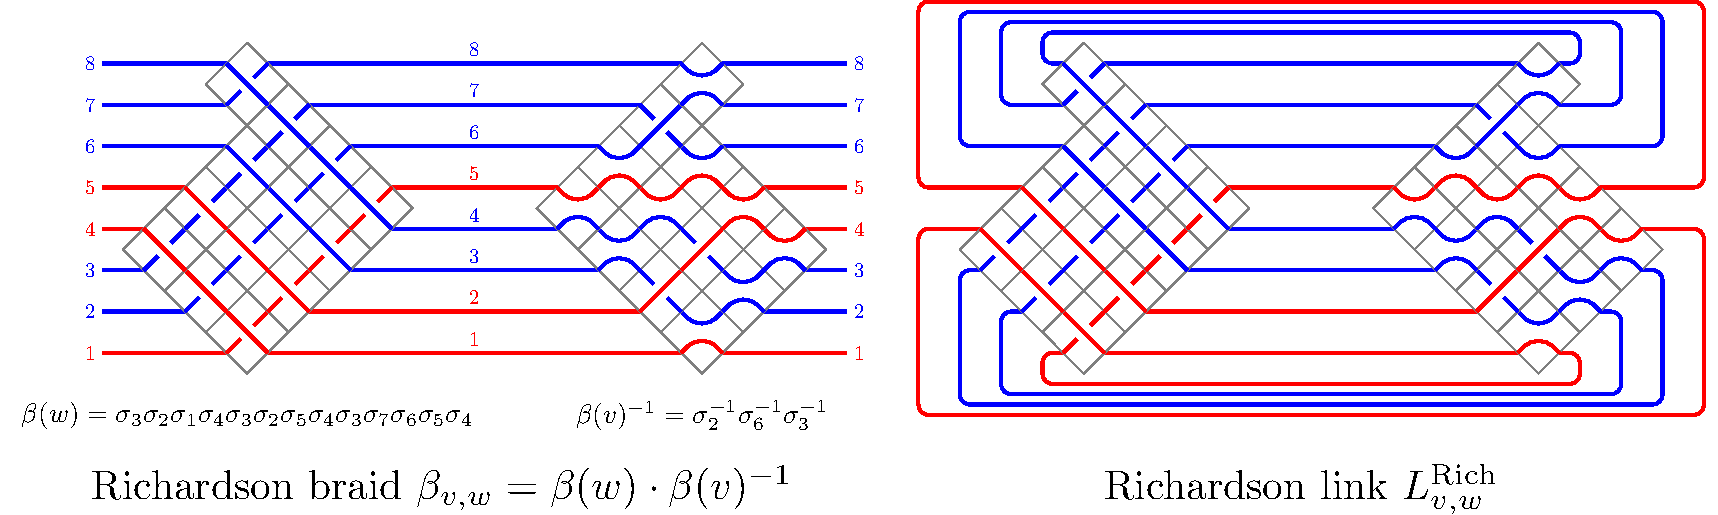
\includegraphics[width=1.0\textwidth]{../assets/840/Lrich.pdf}
  \caption{\label{fig:Lrich} A Richardson braid (left) and a Richardson link (right) defined in \cref{sec:intro:Rich_link}.}
\end{figure}


\subsubsection{Richardson link}\label{sec:intro:Rich_link} A permutation $w\in\Sn$ is called \emph{$k$-Grassmannian} if $w(1)<\cdots<w(\n-k)$ and $w(\n-k+1)<\cdots<w(\n)$. We denote by $\Skn$ the set of $k$-Grassmannian permutations. The permutation $\fp$ can be uniquely decomposed as the product $\fp=wv^{-1}$ for some $1\leq k\leq \n-1$ and some pair $(v,w)\in \Sn\times\Skn$ such that $v\leq w$ in the Bruhat order on~$\Sn$; see \cref{cor:KLS}. For the permutation $\fp$ given by~\eqref{eq:intro:fp}, we get that $k=4$ and\footnote{Our convention for multiplying permutations is right-to-left, i.e.  $\fp(j)=w(v^{-1}(j))$ for all $j\in[\n]$.}
\begin{equation*}%
v=\left(\!\!\text{
\begin{tabular}{cccccccc}
\textcolor{red}{$1$} & \textcolor{red}{$2$} & \textcolor{blue}{$3$} & \textcolor{blue}{$4$} & \textcolor{red}{$5$} & \textcolor{blue}{$6$} & \textcolor{blue}{$7$} & \textcolor{blue}{$8$}\\
\textcolor{red}{$1$} & \textcolor{red}{$4$} & \textcolor{blue}{$2$} & \textcolor{blue}{$3$} & \textcolor{red}{$5$} & \textcolor{blue}{$7$} & \textcolor{blue}{$6$} & \textcolor{blue}{$8$}
\end{tabular}
}\!\!\right)
,\quad
w=\left(\!\!\text{
\begin{tabular}{cccccccc}
\textcolor{red}{$1$} & \textcolor{red}{$2$} & \textcolor{blue}{$3$} & \textcolor{blue}{$4$} & \textcolor{red}{$5$} & \textcolor{blue}{$6$} & \textcolor{blue}{$7$} & \textcolor{blue}{$8$}\\
\textcolor{red}{$4$} & \textcolor{red}{$5$} & \textcolor{blue}{$6$} & \textcolor{blue}{$8$} & \textcolor{red}{$1$} & \textcolor{blue}{$2$} & \textcolor{blue}{$3$} & \textcolor{blue}{$7$}
\end{tabular}
}\!\!\right)
.
\end{equation*}
%
Here, the colors represent the cycles of $\fp=wv^{-1}$. 
 Let $\beta(v),\beta(w)$ be the positive braid lifts of $v,w$ to the braid group of $\Sn$. Consider the \emph{Richardson braid} $\beta_{v,w}:=\beta(w)\cdot \beta(v)^{-1}$ shown in \figref{fig:Lrich}(left). Taking the \emph{braid closure} of $\beta_{v,w}$, we obtain the \emph{Richardson link} $\Lrich_{v,w}=\Lrich_\fp$ shown in \figref{fig:Lrich}(right). We orient the strands of $\beta_{v,w}$ from right to left; cf. \figref{fig:Lrich-to-L'}(left).
%
\begin{remark}\label{rmk:Rich_Young}
It is well known (cf. \cref{sec:Le-diags}) that $k$-Grassmannian permutations are in bijection with Young diagrams that fit inside a $k\times (\n-k)$ rectangle. Thus, in \figref{fig:Lrich}(left), we arrange the crossings in $\beta(w)$ into a (rotated) Young diagram. The condition that $v\leq w$ in the Bruhat order implies that a reduced word for $v$ is a subword of a reduced word for $w$, and thus we represent $\beta(v)^{-1}$ in \figref{fig:Lrich}(left) by replacing some of the crossings in $\beta(w)^{-1}$ with ``elbows.''
%
\end{remark}

 The above recipe was used in~\cite{GL_qtcat} more generally for pairs $v\leq w$ where $w$ is not necessarily $k$-Grassmannian. 

\begin{figure}
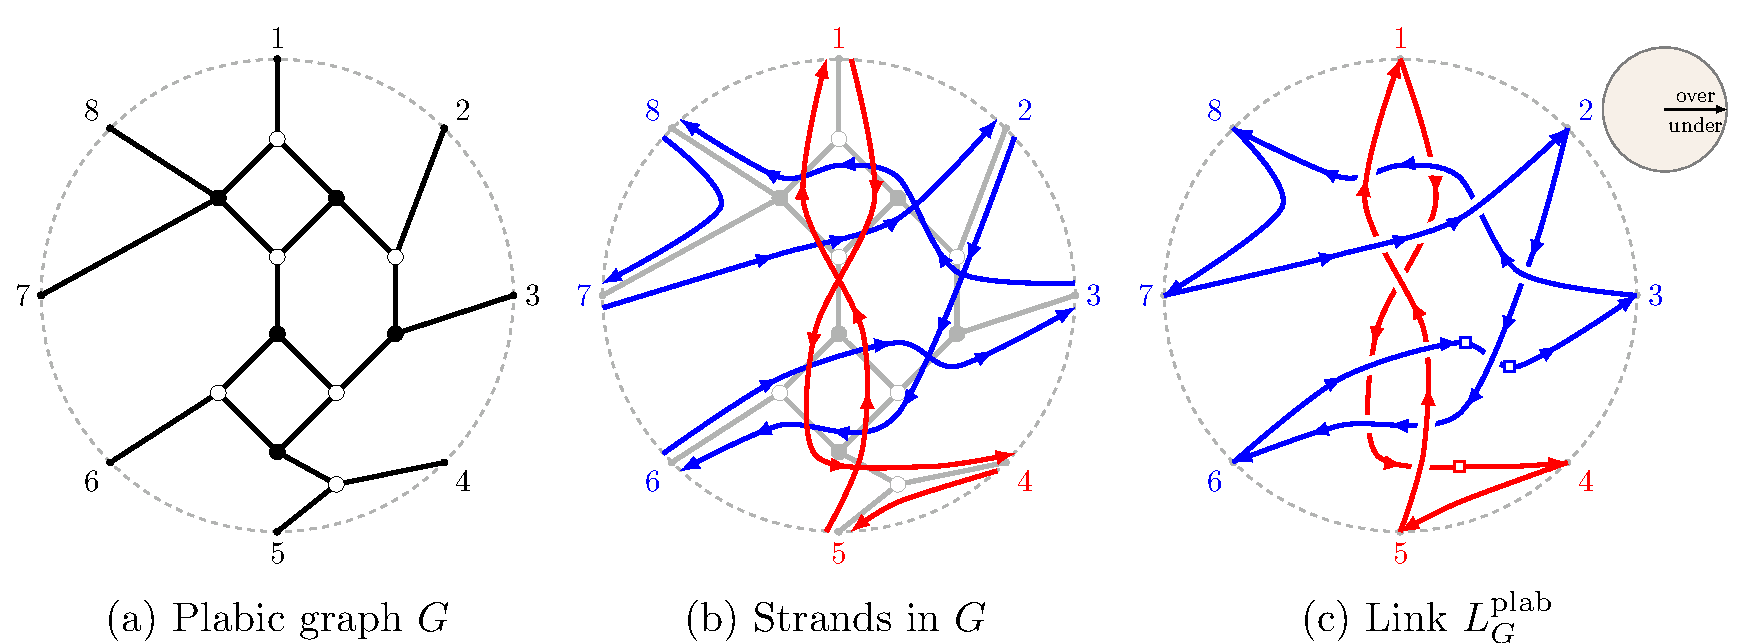
\includegraphics[width=1.0\textwidth]{../assets/840/Lplab.pdf}
  \caption{\label{fig:Lplab} Converting a plabic graph $G$ into the plabic graph link $\Lplab_G$.}
\end{figure}


\subsubsection{Plabic link} \label{sec:intro:plabic_link}
%
A \emph{plabic graph} is a non-empty planar graph $G$ embedded in a disk with vertices colored black and white; see~\cite{Pos}.  
%
 A \emph{strand} in $G$ is a path that makes a sharp right turn at each black vertex and a sharp left turn at each white vertex. We assume that the graph $G$ has $\n$ boundary vertices, all of which have degree $1$ and are labeled $1,2,\dots,\n$ in clockwise order. An example of a plabic graph $G$ is shown in \figref{fig:Lplab}(a), and the strands in $G$ are shown in \figref{fig:Lplab}(b).

The following description of the \emph{plabic graph link} $\Lplab_G$, or \emph{plabic link} for short, can be deduced from~\cite{ACampo,STWZ,FPST} by breaking the symmetry following~\cite{Hirasawa}. (See \cref{sec:plabic_links_properties} for a more invariant description.) The planar diagram of $\Lplab_G$ will consist of the union of the strands of $G$. To specify the overcrossings, let $p$ be an intersection point of two strands $S_1,S_2$ in $G$.  The tangent vector to $S_1$ (resp. $S_2$) at $p$ can be considered a vector in the complex plane, and we let $\Arg(S_1,p) \in[0,2\pi)$ (resp. $\Arg(S_2,p)\in[0,2\pi)$) denote the argument of this vector.
%
We assume that $0<\Arg(S_1,p)\neq\Arg(S_2,p)<2\pi$. Then $S_1$ is drawn above $S_2$ if $\Arg(S_2,p)>\Arg(S_1,p)$, otherwise $S_1$ is drawn below $S_2$. 

\begin{figure}
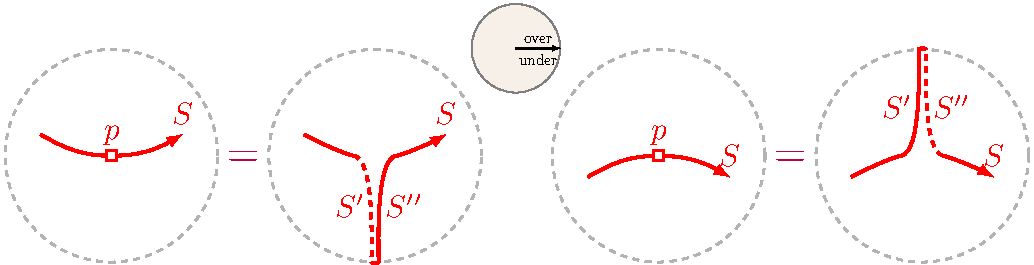
\includegraphics[width=0.7\textwidth]{../assets/840/over_under.pdf}
  \caption{\label{fig:over_under} For every point $p$ on a strand $S$ satisfying $\Arg(S,p)=0$, we insert a strand segment going to the boundary and back; see \cref{sec:intro:plabic_link}.}
\end{figure}



A technical extra step is required to finalize the construction of $\Lplab_G$; see \cref{fig:over_under}. Consider a point $p$ on a strand $S$ such that $\Arg(S,p)=0$, i.e.  such that $S$ is directed to the right at $p$. We add an extra segment $S'$ to $S$ traveling from $p$ to the boundary of the disk followed by a segment $S''$ traveling from the boundary back to $p$. In the neighborhood of $p$, $S$ looks like a plot of a function. If this function is ``concave up'' at $p$ (i.e.  has positive second derivative), then $S'$ (resp. $S''$) is drawn below (resp. above) all other strands. If $S$ is ``concave down'' at $p$ then $S'$ (resp. $S''$) is drawn above (resp. below) all other strands. 

Finally, each boundary vertex of $G$ is an endpoint of exactly two strands (one outgoing and one incoming). We join these endpoints together and obtain a planar diagram of a link denoted $\Lplab_G$. See \figref{fig:Lplab}(c), where the points $p$ such that $\Arg(S,p)=0$ are marked by the symbol $\mysq$.

 The strands in $G$ that start and end at the boundary vertices give rise to the \emph{strand permutation} $\pig$ of $G$. In this subsection, we will assume that $G$ is \emph{reduced}, i.e.  that $G$ has the minimal possible number of faces among all graphs with a given strand permutation. Importantly, in \cref{sec:intro:quivers-point-count}, we will drop this assumption. Postnikov~\cite{Pos} showed that for any $\pi\in \Sn$, there exists a reduced plabic graph $G$ with strand permutation $\pig=\pi$. For example, for $\pi$ given by~\eqref{eq:intro:fp}, one can take $G$ to be the graph in \figref{fig:Lplab}(a). Up to isotopy, the resulting link $\Lplab_G$ depends only on $\pi$ and is denoted $\Lplab_\pi$. 

%
%
%

%


%
%


\begin{figure}
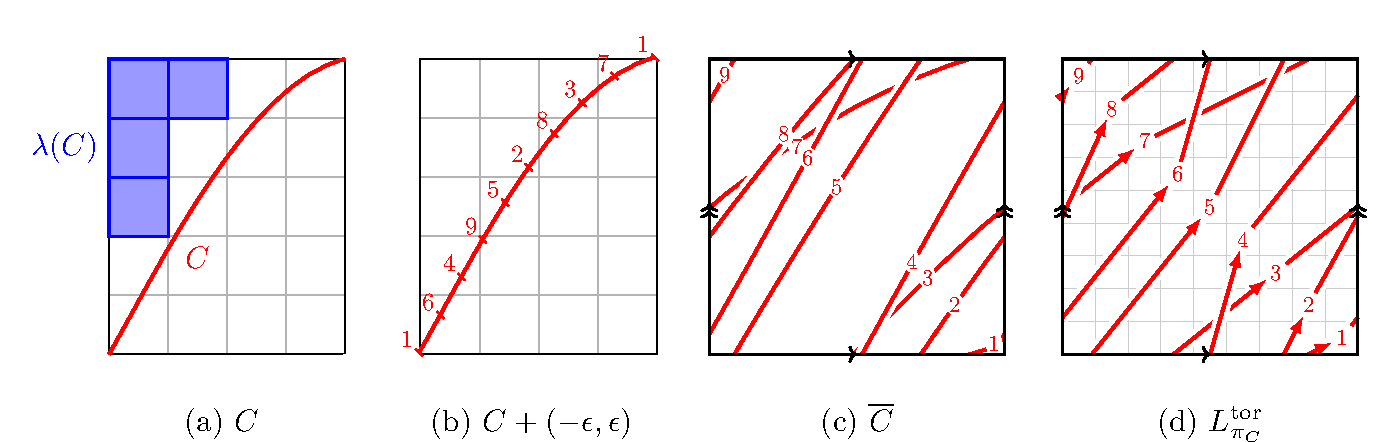
\includegraphics[width=1.0\textwidth]{../assets/840/concave_1.pdf}
  \caption{\label{fig:concave} Converting a concave curve $C$ into the link $\Ltor_{\pi_C}$ for some $\pi_C\in\Sn$; see \cref{ex:intro:Cox}.}
\end{figure}


\subsubsection{Coxeter link} \label{sec:intro:cox_link}
In~\cite[Section~6]{GL_cat_combin}, we studied \emph{concave permutations}, defined as follows. Choose a generic concave curve $C$ inside a $k\times (\n-k)$ rectangle connecting $(0,0)$ to $(\n-k,k)$ as in \figref{fig:concave}(a). We will shift it by the vector $(-\eps,\eps)$ for some small $\eps>0$ as in \figref{fig:concave}(b). Under the natural projection $\R^2\to\T=\R^2/\Z^2$, the curve $C+(-\eps,\eps)$ projects to a curve $\Cproj$ in the unit square $[0,1]^2$. For each self-intersection of $\Cproj$, we draw the segment of the higher slope above the segment of the lower slope; see \figref{fig:concave}(c). The resulting link diagram is isotopic to $\Ltor_\pi$ for a permutation $\pi=\pi_C\in\Sn$ which can be explicitly read off from $\Cproj$ as follows. Label the intersection points of $\Cproj$ with the $y=1-x$ diagonal of $[0,1]^2$ by $d_1,d_2,\dots,d_\n$, proceeding in the northwest direction. Thus, $d_1=(1-\eps,\eps)$ is the projection of the starting and ending points of $C+(-\eps,\eps)$. In \figref{fig:concave}(c), we represent each point $d_i$ by~$i$. Since $C$ was generic, we assume that the points $d_1,d_2,\dots, d_\n$ are pairwise distinct. The permutation $\pi_C$ is defined so that each segment of $C$ connects (in the northeast direction) $d_i$ to $d_{\pi(i)}$ for some $i\in[\n]$. See \figref{fig:concave}(d). We refer to permutations that can be obtained in this way as \emph{concave permutations}. They form a subclass of the class of \emph{repetition-free permutations} introduced in~\cite{GL_cat_combin}.

Let $\la_C=(\la_1,\la_2,\dots,\la_k)$ be the Young diagram inside the $k\times (\n-k)$ rectangle consisting of all unit boxes strictly above $C$, shown in \figref{fig:concave}(a). 
%
 Consider a sequence $\abf(C)=(a_2,\dots,a_k)$ given by $a_i:=\la_{i-1}-\la_i$ for $2\leq i\leq k$. The \emph{Coxeter link} $\Lcox_C$ is the closure of the braid
\begin{equation}\label{eq:beta_abf_dfn}
  \beta(\abf(C)):=\ell_2^{a_2}\cdots \ell_k^{a_k}\cdot\sigma_1\cdots \sigma_{k-1},
\end{equation}
where $\sigma_1,\dots,\sigma_{k-1}$ are the standard braid group generators of the braid group of $S_k$, and $\ell_i=\sigma_{i-1}\cdots \sigma_1\cdot \sigma_1\cdots \sigma_{i-1}$ are the Jucys--Murphy elements. 

\begin{figure}
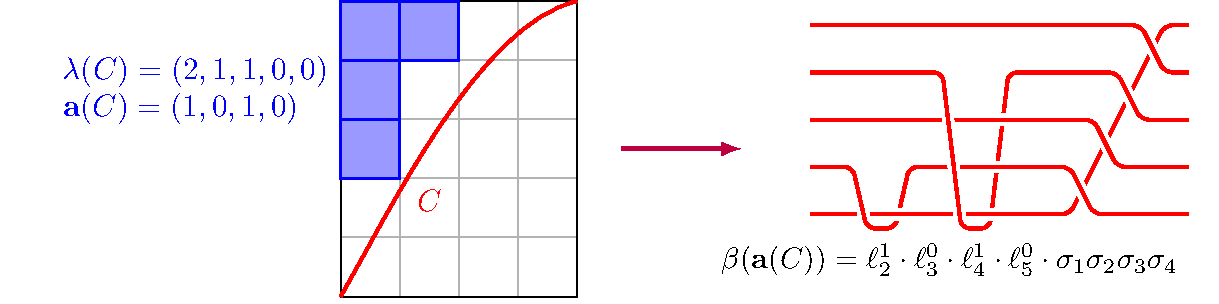
\includegraphics[width=0.85\textwidth]{../assets/840/concave_2.pdf}
  \caption{\label{fig:concave_2} Converting a concave curve $C$ into the Coxeter braid $\beta(\abf(C))$.}
\end{figure}
\begin{example}\label{ex:intro:Cox}
Let $C$ be the curve shown in \cref{fig:concave,fig:concave_2}. We have $k=5$ and $\n=9$. The permutation $\pi_C=\left(\!\!\text{
\begin{tabular}{ccccccccc}
%
%
$1$ & $2$ & $3$ & $4$ & $5$ & $6$ & $7$ & $8$ & $9$\\
$6$ & $8$ & $7$ & $9$ & $2$ & $4$ & $1$ & $3$ & $5$
\end{tabular}
}\!\!\right)$ can be read off from the labels\footnote{The labels in \figref{fig:concave}(b) are chosen in such a way that when we project $C$ to the unit square, they become ordered along the diagonal $y=1-x$; see \figref{fig:concave}(c).} in \figref{fig:concave}(b): in cycle notation, $\pi_C$ is given by $\pi_C=(1\,6\,4\,9\,5\,2\,8\,3\,7\,1)$. We have $\la_C=(2,1,1,0,0)$, $\abf(C)=(1,0,1,0)$,  and $\beta(\abf(C))=\ell_2\ell_4\sigma_1\sigma_2\sigma_3\sigma_4$; see also~\cite[Figure~13]{GL_cat_combin}.
\end{example}
%
 Coxeter links and their Khovanov--Rozansky homology have previously been studied in relation to flag Hilbert schemes and generalized shuffle conjectures~\cite{ObRo,GN,GNR,BHMPS}; see also~\cite[Section~7.2]{GL_cat_combin}.
%
 %
%
%

The following is our first main result.
\begin{theorem}\label{thm:isotopy}
  Let $\fp\in\Sn$ be a permutation without fixed points. Then the links $\Lperm_\fp$, $\Ltor_\fp$, $\Lrich_\fp$, and $\Lplab_\fp$ are all isotopic. If $\fp=\fp_C$ for some concave curve $C$ then each of these links is also isotopic to $\Lcox_C$.
%
\end{theorem}
We refer to any one of the above links as the \emph{positroid link} of $\fp$.

%
%
%

%

%


\begin{remark}
The recent work~\cite{CGGS} independently constructs Legendrian isotopies (a stronger result than our smooth isotopies) between the Richardson link $\Lrich_\pi$ and other closely related links: closures of juggling braids, cyclic rank matrix braids, and Le-diagram braids.  We expect the Le-diagram braid in~\cite{CGGS} to be closely related to our plabic graph link $\Lplab_\fp$, and the juggling braid to be similar to our permutation link $\Lperm_\fp$, though we believe our definition of $\Lperm_\fp$ is the simplest and most elementary.

Isotopies between cyclic rank matrix links and plabic graph links have also been observed in~\cite{STWZ}.
%
%
\end{remark}

\subsection{Quiver point count and the HOMFLY polynomial}\label{sec:intro:quivers-point-count}
In this subsection, we consider not necessarily reduced plabic graphs $G$. Throughout the paper, we assume that the interior faces of $G$ are simply connected, i.e.  that no interior face of $G$ contains another connected component of $G$ inside of it. For simplicity, we also assume that each plabic graph $G$ is \emph{trivalent}, i.e.  that each interior vertex of $G$ has degree $3$. (Recall that the boundary vertices of $G$ are always required to have degree $1$.) This is not a restrictive assumption: any vertex of degree $2$ in $G$ can be omitted (joining two of its neighbors by an edge), and any vertex of degree higher than $3$ in $G$ can be ``uncontracted'' into several vertices of degree $3$ of the same color; see~\cite[Figure~12.2]{Pos}.
%
%
%
%

Let $G$ be a (trivalent) plabic graph. The planar dual of $G$ naturally contains a directed (sub)graph denoted $\QG$. Explicitly, place a vertex of $\QG$ inside each \emph{interior face} of $G$ (i.e.  a face not incident to the boundary of the disk). For every edge $e$ of $G$ whose endpoints are of different color and such that the two faces $F,F'$ incident to $e$ are both interior, $\QG$ contains an arrow between $F$ and $F'$. (These two faces $F,F'$ may or may not be equal.) The direction of the arrow is chosen so that the white endpoint of $e$ is on the left as one moves along this arrow. See \cref{fig:simple}.


\begin{figure}
  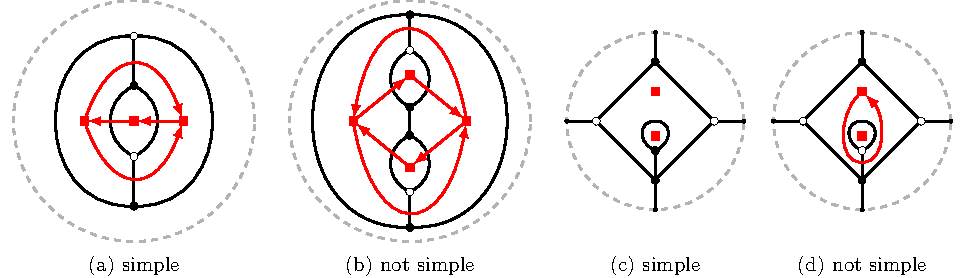
\includegraphics[width=1.0\textwidth]{../assets/840/simple.pdf}
  \caption{\label{fig:simple} Examples of simple and non-simple plabic graphs $G$ (black) and the associated quivers $\QG$ (red).}
\end{figure}

%
 The following definition is crucial for our analysis.
\begin{definition}
A plabic graph $G$ is called \emph{simple} if the directed graph $\QG$ is a \emph{quiver}, i.e.  contains no directed cycles of length $1$ and $2$.
\end{definition}
For example, the plabic graph $G$ in \figref{fig:simple}(b) is not simple since $\QG$ contains a pair of opposite arrows. The graph $G$ in \figref{fig:simple}(d) is not simple since $\QG$ contains a loop arrow. The graphs in \figref{fig:simple}(a,c) are simple.
%

%

%


%

To every \emph{\Louise} quiver $Q$ (see~\cref{sec:quiver}), we associate a rational function $\RQ(q)$ called the \emph{point count rational function}. It can be computed via an explicit recurrence relation: see~\eqref{eq:RQ_recurrence} and~\eqref{eq:RQ_skein}. The function $\RQ(q)$ has the following interpretation in terms of \emph{cluster algebras}~\cite{FZ}; see~\cref{sec:quiver} for the relevant definitions. 
Let $Q$ be a quiver with $n$ vertices. Consider an ice quiver $\Qice$ with $m$ frozen vertices and mutable part $Q$, and assume that the rows of the $(n+m)\times n$ exchange matrix $\BQice$ of $\Qice$ span $\Z^n$ over $\Z$. Then the cluster algebra $\AQice$ gives rise to a \emph{cluster variety} $\XQice$, and its point count over a finite field $\F_q$ with $q$ elements (for $q$ a prime power) is given by
\begin{equation*}%
  \#\XQice(\F_q)=(q-1)^m\cdot \RQ(q);
\end{equation*}
see \cref{prop:Q_pcnt}.

%
%

 A typical example of this phenomenon occurs when $G$ is a reduced plabic graph: then, by~\cite{GL_cluster}, 
 %
%
  $\AQGice$ is the coordinate ring of the associated \emph{open positroid variety} $\Pio_G$ inside the Grassmannian~\cite{Pos,KLS}. In particular, $(q-1)^{\n-\conn(G)}\RQG(q)$ counts the number of points in $\Pio_G(\F_q)$, where $\n$ is the number of boundary vertices of $G$ and $\conn(G)$ is the number of connected components of $G$.%

Given an (oriented) link $L$, one can define a Laurent polynomial $\HOMP(L)=\HOMP(L;a,z)$ called the \emph{\FLY polynomial}~\cite{HOMFLY,PT} of $L$. It is defined by the skein relation
\begin{equation}\label{eq:HOMFLY_dfn}
  %
  a\HOMP(L_+) - a^{-1} \HOMP(L_-)=z\HOMP(L_0)\quad \text{and}\quad \HOMP(\unknot)=1.
\end{equation}
Here, $\unknot$ denotes the unknot and  $L_+$, $L_-$, $L_0$ are any three links whose planar diagrams locally differ as  follows.
\newcommand\lw{3pt}
\newcommand\lww{10pt}
\newcommand\drcirc{
\draw[line width=0.3pt, dashed] (0,0) circle (1cm);
}
\newcommand\scl{0.4}

\newcommand\DA{30}
\begin{center}
\begin{tabular}{ccc}
\scalebox{\scl}{
\begin{tikzpicture}
\drcirc
\draw[line width=\lw,->,>=latex] (-90+\DA:1)--(90+\DA:1);
\draw[line width=\lww,white] (-90-\DA:1)--(90-\DA:1);
\draw[line width=\lw,->,>=latex] (-90-\DA:1)--(90-\DA:1);
\end{tikzpicture}
} 

& 

 
\scalebox{\scl}{ 
\begin{tikzpicture}
\drcirc
\draw[line width=\lw,->,>=latex] (-90-\DA:1)--(90-\DA:1);
\draw[line width=\lww,white] (-90+\DA:1)--(90+\DA:1);
\draw[line width=\lw,->,>=latex] (-90+\DA:1)--(90+\DA:1);
\end{tikzpicture} 
} 
& 
 
\newcommand\rc{10} 
\scalebox{\scl}{ 
\begin{tikzpicture}
\drcirc
\draw[line width=\lw,->,>=latex,rounded corners=\rc] (-90-\DA:1)--(0,0)--(90+\DA:1);
\draw[line width=\lw,->,>=latex,rounded corners=\rc] (-90+\DA:1)--(0,0)--(90-\DA:1);
\end{tikzpicture} 
} 
\\ 
$L_+$  &  $L_-$  &  $L_0$

  

\end{tabular}
\end{center}
For a (not necessarily reduced) plabic graph $G$ we let $\Lplab_G$ be the corresponding plabic graph link, defined as in \cref{sec:intro:positroid_links}. Following~\cite{GL_qtcat}, we let  $\Ptop_L(q)$ be obtained from the top $a$-degree term of $\HOMP(L;a,z)$ by substituting $a:=q^{-\frac12}$ and $z:=q^{\frac12}-q^{-\frac12}$. The following conjecture generalizes~\cite[Theorem~1.11]{GL_qtcat} (see also~\cite{STZ,STWZ}).
\begin{conjecture} \label{conj:main}
Let $G$ be a simple plabic graph with $\conn(G)$ connected components.  Then we have
\begin{equation}\label{eq:FLY=pcnt}
  \RQG(q)= (q-1)^{\conn(G)-1}\Ptop_{\Lplab_G}(q).
\end{equation}
%
\end{conjecture}
For examples, see Figure~9, Example~5.12, and Section~9.

When the plabic graph $G$ is reduced, \cref{conj:main} becomes~\cite[Theorem~1.11]{GL_qtcat}. We present a different proof in \cref{sec:sub_skein-relation} by giving a plabic graph interpretation of the \FLY skein relation~\eqref{eq:HOMFLY_dfn}. More generally, in \cref{sec:leaf-recurr-plab}, we introduce a class of \emph{leaf recurrent plabic graphs} and prove \cref{conj:main} for them. 

%
 %
%
%
%
\begin{theorem}\label{thm:FLY=pcnt_leaf_rec}
  \Cref{conj:main} holds for leaf recurrent plabic graphs.
\end{theorem}
 %
 The fact that reduced plabic graphs are leaf recurrent was shown in~\cite[Remark~4.7]{MSLA}. Another natural subclass of leaf recurrent plabic graphs are the \emph{plabic fences} of~\cite[Section~12]{FPST}.
%
 A \emph{plabic fence} is a plabic graph obtained by drawing $k$ horizontal strands and inserting an arbitrary number of black-white and white-black bridges between them; see \cref{fig:plabic_fence} for an example and \cref{sec:plabic-fences} for a precise definition.
%
\begin{figure}
  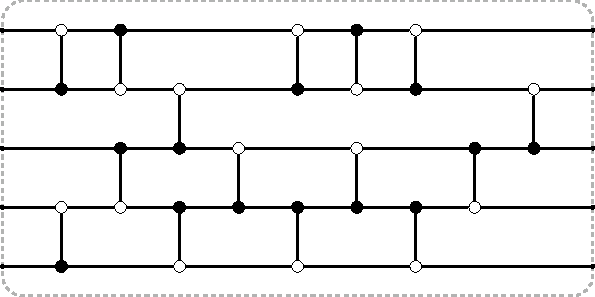
\includegraphics[width=0.5\textwidth]{../assets/840/plabic_fence.pdf}
  \caption{\label{fig:plabic_fence} A plabic fence.}
\end{figure}


\begin{proposition}\label{prop:reduced_and_fence_are_leaf_rec}
Reduced plabic graphs and plabic fences are leaf recurrent. In particular, \cref{conj:main} holds for these classes of plabic graphs.
\end{proposition}
%
This result gives a new proof of~\cite[Theorem~1.11]{GL_qtcat}.

A primary difficulty in showing \cref{conj:main} in full generality comes from the examples described in Sections~9.1 and~9.2. Section~9.1 explains that the simple plabic graph $G$ in \figref{fig:simple}(a) is not leaf recurrent. The quiver $\QG$ is \Louise (in fact, it is mutation equivalent to an acyclic quiver), and thus the point count polynomial $\RQG(q)$ can be easily checked to coincide with $\Ptop_{\Lplab_G}(q)$. Section~9.2 describes a simple plabic graph $G$ such that $\QG$ is not locally acyclic, in which case the task of computing $\RQG(q)$ becomes much harder.
%

Both sides of~\eqref{eq:FLY=pcnt} are rational functions in $q$ which are specializations of rational functions in $(q,t)$ arising from the cohomology of cluster varieties on the one hand and Khovanov--Rozansky link homology on the other hand. Thus, one can make a stronger conjecture where both sides of~\eqref{eq:FLY=pcnt} become polynomials in $(q,t)$. We discuss this in more detail in Section~8.3.
% We discuss these more general conjectures in Section~8.3.
%

\begin{remark}
In special cases, the cluster point count rational function $R(Q;q)$ has an explicit combinatorial description as a positive sum of terms of the form $(q-1)^a q^b$.  This holds, for example, when $Q$ is acyclic \cite{LS2} (see \cref{prop:acycliccount}), or when the cluster variety is a Richardson variety \cite{Deodhar}, see also \cite[Section 9]{GL_qtcat}.    We remark that such formulae should be compared to ruling polynomials of links \cite{Ruth}, though we do not know such a formula for general plabic graph quivers $Q_G$.
\end{remark}

\section{Positroid combinatorics}\label{sec:positr-comb}
In this section, we review some background on the combinatorics of plabic graphs and the associated objects.


\subsection{Bounded affine permutations}\label{sec:bound-affine-perm}
A \emph{$(k,\n)$-bounded affine permutation}~\cite{KLS} is a bijection $f:\Z\to\Z$ such that 
\begin{itemize}
\item $f$ is \emph{$\n$-periodic}: $f(i+\n)=f(i)+\n$ for all $i\in \Z$,
\item  $i\leq f(i)\leq i+\n$ for all $i\in\Z$, and %
\item $\sum_{i=1}^\n(f(i)-i)=k\n$.
\end{itemize}
The set of $(k,\n)$-bounded affine permutations is denoted $\Boundkn$. Each $f\in\Boundkn$ gives rise to a unique permutation $\fbar\in\Sn$ defined by $\fbar(i)\equiv f(i)\pmod \n$ for each $i\in[\n]$. Given $f\in\Boundkn$, an integer $i\in\Z$ is called a \emph{loop} (resp. a \emph{coloop}) of $f$ if $f(i)=i$ (resp. $f(i)=i+\n$). Thus, $\fbar$ has no fixed points if and only if $f$ has no loops and no coloops. In this case, $f$ is uniquely determined by $\fbar$, and the integer $k$ is recovered from $\fbar$ as follows:
\begin{equation*}%
  k=k(\fbar):=\#\{i\in[\n]\mid \fbar(i)<i\}.
\end{equation*}
We define $\taukn\in\Boundkn$  by
\begin{equation*}%
  \taukn(i)=
  \begin{cases}
    i, &\text{if $1\leq i\leq \n-k$,}\\
    i+\n, &\text{if $\n-k+1\leq i\leq \n$,}
  \end{cases}
\end{equation*}
and extend it to a function $\taukn:\Z\to\Z$ by $\n$-periodicity. 


Let $\Qkn:=\{(v,w)\in \Sn\times \Skn\mid v\leq w\}$, where $\leq$ denotes the Bruhat order on $\Sn$. Given a permutation $u\in\Sn$, we can extend it to an $\n$-periodic map $\tilde u:\Z\to\Z$ defined by $\tilde u(i)=u(i)$ for $i\in[\n]$. For $(v,w)\in\Qkn$, let $f_{v,w}:=\tilde w\taukn\tilde v^{-1}$. By~\cite[Proposition~3.15]{KLS}, the map $(v,w)\mapsto f_{v,w}$ gives a bijection $\Qkn\xrightarrow{\sim} \Boundkn$. Taking the inverse of this map, we obtain the following result, justifying the definition of a Richardson link in \cref{sec:intro:Rich_link}.
\begin{corollary}\label{cor:KLS}
If $\fp\in\Sn$ has no fixed points then it can be uniquely factored as a product $\fp=wv^{-1}$, where $(v,w)\in\Qkn$ and $k=k(\fp)$.
\end{corollary}

The open positroid stratification~\cite{KLS} of the Grassmannian contains a unique open dense stratum. It is labeled by the bounded affine permutation $\fkn\in\Boundkn$ sending $i\mapsto i+k$ for all $i\in\Z$. We let $\pikn\in\Sn$ be the permutation sending $i\mapsto i+k$ modulo $\n$ for all $i\in[\n]$.


\subsection{Plabic graphs}\label{sec:plabic-graphs}
%
%
%
%
%
%
%
%
%
%
%

\begin{figure}
  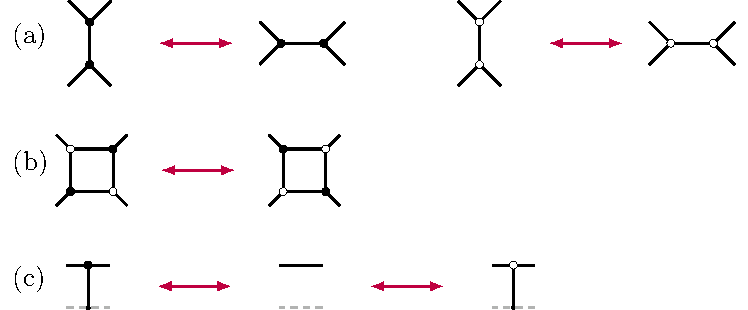
\includegraphics[width=0.7\textwidth]{../assets/840/moves.pdf}
  \caption{\label{fig:moves} Local moves for plabic graphs: (a) contraction-uncontraction move; (b) square move; (c) tail addition/removal.}
\end{figure}




%

%

Let $G$ be a plabic graph. Recall from \cref{sec:intro:plabic_link} that $G$ must be nonempty, that the boundary vertices of $G$ are labeled by $1,2,\dots,\n$ in clockwise order, and that the strand permutation $\pig:[\n]\to[\n]$ sends $i\mapsto j$ whenever the strand starting at $i$ terminates at $j$. We always assume that our plabic graphs $G$ are such that $\pig$ has no fixed points, although most of our constructions can be easily extended to this case; see Section~4.5.

%

\begin{definition}[\cite{Pos}]
We say that $G$ is \emph{reduced} if it has the minimal number of faces among all plabic graphs with strand permutation $\pig$.
\end{definition}
Alternatively~\cite[Theorem~13.2]{Pos}, a plabic graph $G$ is reduced if and only if $G$ has no closed strands, no self-intersecting strands, and no pairs of strands forming a \emph{bad double crossing} shown in \figref{fig:double}(right). \emph{Good double crossings} shown in \figref{fig:double}(left) are allowed.

We consider several types of \emph{local moves} on plabic graphs, shown in \cref{fig:moves}. 
%
 It was shown in~\cite{Pos} that every permutation $\pi\in\Sn$ is the strand permutation of some reduced plabic graph $G$, and that moreover, any two reduced plabic graphs with the same strand permutation are related by a sequence of the moves (a) and (b) in \cref{fig:moves}. Below we review one construction of plabic graphs which will be particularly useful to us.

\subsection{Le-diagrams}\label{sec:Le-diags}
Let $\la=(\la_1\geq\la_2\geq\cdots\geq\la_k\geq0)$ be a partition, which we identify with its Young diagram. We assume that this Young diagram fits inside a $k\times (\n-k)$ rectangle, i.e.  satisfies $\la_1\leq \n-k$. We draw Young diagrams using \emph{English} (or \emph{matrix}) \emph{notation}. We use matrix coordinates for the boxes of $\la$, thus, row $i$ contains boxes with coordinates $(i,j)$ for $1\leq j\leq \la_i$, and box $(1,1)$ is the top left box.

A \emph{Le-diagram} $\Gamma$ \emph{of shape $\la$} is a way of placing a dot in some of the boxes of $\la$ so that every box that is below a dot in the same column and to the right of a dot in the same row must also contain a dot.  
%
 An example of a Le-diagram of shape $\la=(3,3,3,1)$ is shown in \figref{fig:Gamma-to-L'}(left). Le-diagrams whose shape fits inside a $k\times(\n-k)$ rectangle are in bijection with the elements of $\Qkn$ and $\Boundkn$; see~\cite[Section~19]{Pos}. Given a Le-diagram $\Gamma$ of shape $\la$, one can read off the corresponding pair $(v,w)\in\Qkn$ as follows. First, $w\in\Skn$ is the $k$-Grassmannian permutation corresponding to $\la$. Specifically, let us label the unit steps in the southeast boundary of $\la$ by $1,2,\dots,\n$ in increasing order from the northeast to the southwest corner. Then the labels of the vertical steps form a $k$-element subset of $[\n]$, and this set is precisely $\{w(\n-k+1),\dots,w(\n)\}$. This determines $w$ uniquely. Alternatively, we can label each box $(i,j)$ of $\la$ with the simple transposition $s_{k+j-i}$, and then a reduced word for $w$ is obtained by reading these simple transpositions in the northwest direction. Thus, any reduced word for $w$ ends with $s_k$ which labels the box $(1,1)$. To obtain a reduced word for $v$, we read these simple transpositions but ignore the ones labeled by dots in $\Gamma$. Conversely, given $(v,w)\in\Qkn$, the shape $\la$ of $\Gamma$ is reconstructed from $w$, and the empty boxes of $\Gamma$ correspond to the rightmost subexpression for $v$ inside the (unique up to commutation) reduced word for $w$.
\begin{example}
For the Le-diagram in \figref{fig:Gamma-to-L'}(left), we have 
\begin{equation*}%
w= s_7 s_3 s_4 s_5 s_6 s_2 s_3 s_4 s_5 s_1 s_2 s_3 s_4
\quad\text{and}\quad
v= s_6 s_3 s_2.
\end{equation*}
\end{example}

\begin{figure}
  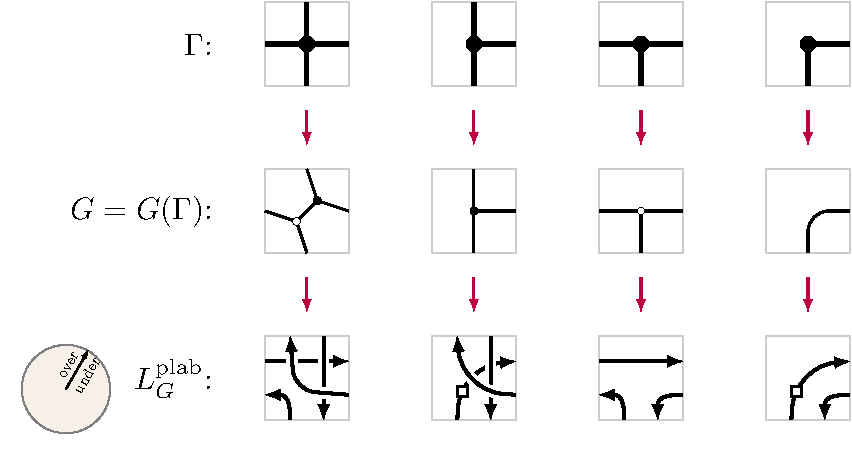
\includegraphics[width=0.7\textwidth]{../assets/840/Le_to_G.pdf}
  \caption{\label{fig:Le_to_G} Converting a Le-diagram (top row) into a plabic graph (middle row) and into a link (bottom row).}
\end{figure}



A Le-diagram $\Gamma$ can be converted into a plabic graph $G(\Gamma)$ using the local rules shown in the first two rows of \cref{fig:Le_to_G}. This plabic graph is always reduced and has strand permutation $\fp=wv^{-1}$, where $(v,w)\in\Qkn$ are recovered from $\Gamma$ using the above procedure.


%

\subsection{Properties of plabic graph links}\label{sec:plabic_links_properties}
Let $G$ be a reduced plabic graph with strand permutation $\pi=\pig$. Recall the description of the plabic graph link $\Lplab_\pi=\Lplab_G$ from \cref{sec:intro:plabic_link}. It may appear from this description that $\Lplab_G$ depends on the precise way of drawing the strands in $G$ as smooth curves, or that $\Lplab_G$ changes if one rotates the graph $G$ (since the over/under-crossings information depends on the complex arguments of the strands). However, it turns out that the link $\Lplab_G$ is in fact independent of these choices, as explained in~\cite{ACampo,STWZ,FPST}. Let us give a more invariant description of $\Lplab_G$.

Recall that $G$ is embedded in a disk $\disk:=\{x\in\C: |x|\leq 1\}$. Consider the solid torus $\disk\times S^1$, and consider an equivalence relation $\sim$ on it defined as follows: for $(x,y),(x',y')\in \disk\times S^1$, write $(x,y)\sim(x',y')$ if $x,x'\in\partial \disk$ belong to the boundary of the disk and $x=x'$. In other words, we collapse each fiber $x\times S^1$, where $x\in\partial \disk$, to a point. The resulting quotient space $\disk\times S^1/\sim$ is homeomorphic to a $3$-dimensional sphere $S^3$.

An \emph{oriented divide} is a smooth immersion of a union of oriented circles (called \emph{branches}) into $\disk$. 
 %
%
%
%
%
 Divides are required to satisfy certain genericity conditions, e.g. that any intersections between the branches must be transversal and belong to the interior of $\disk$, and that there have to be no triple intersections; see~\cite[Definitions~2.1 and~8.1]{FPST} for a complete list. 

Given a branch $\gamma$ of an oriented divide $\Divide$, we lift each point of $\gamma$ to $\disk\times S^1$ by letting the $S^1$ coordinate be the complex argument of the tangent vector of $\gamma$ at this point. By the genericity assumptions, we obtain an embedding of a union of oriented circles into $S^3$, i.e.  a link, denoted $L_\Divide$.

\begin{figure}
  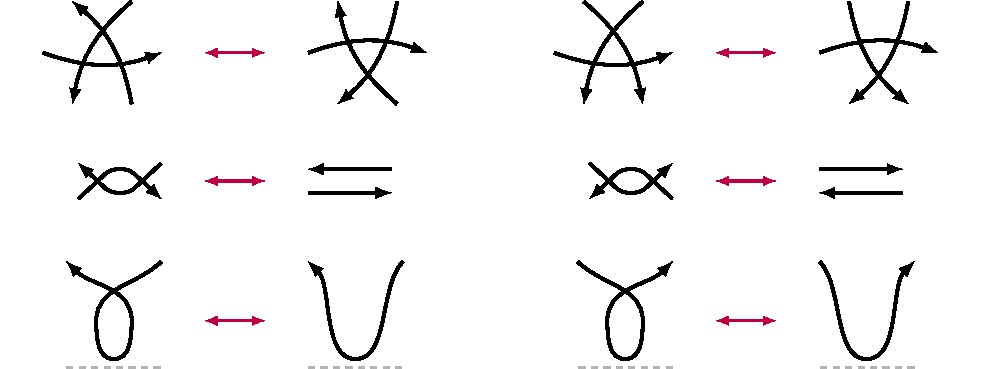
\includegraphics[width=0.7\textwidth]{../assets/840/divide_moves.pdf}
  \caption{\label{fig:divide_moves} Local moves for divides~\cite[Figures~28--30]{FPST}.}
\end{figure}


The link $L_\Divide$ is invariant under applying the local moves shown in \cref{fig:divide_moves} to $\Divide$; see~\cite[Proposition~8.4]{FPST}. We thank the anonymous referee for pointing out that the map $\Divide \mapsto L_\Divide$ coincides with the map reconstructing a Legendrian curve from its front projection. Thus, the invariance under local moves may be deduced from e.g.~\cite{Arnold}.

Take the strands in our reduced plabic graph $G$. Each of the $\n$ boundary vertices of $G$ has one incoming strand and one outgoing strand. Identifying their endpoints, we obtain an oriented divide $\Divide(G)$. It was shown in~\cite{Hirasawa} that the associated link $L_{\Divide(G)}$ is isotopic to the link $\Lplab_G$ described in \cref{sec:intro:plabic_link}. This shows that the link $\Lplab_G$ is indeed invariant under rotation of $G$ and under small perturbations of the branches of $\Divide(G)$, since this is clearly the case for $L_{\Divide(G)}$. 

\begin{remark}\label{rmk:rotation}
In what follows, it will be convenient to us to use rotational invariance of $\Lplab_G$. In our figures, we will fix some angle $\alpha\in[0,2\pi)$, and assume that the link $\Lplab_G$ is obtained by first rotating $G$ by the angle $-\alpha$, then applying the description from \cref{sec:intro:plabic_link}, and then rotating the picture back by $\alpha$. In other words, if two strands $S_1,S_2$ in $G$ intersect at some point $p$, we consider their complex arguments of tangent vectors in a different interval: $\Arg(S_1,p),\Arg(S_2,p)\in[\alpha,\alpha+2\pi)$. Then we draw $S_1$ above $S_2$ if and only if $\Arg(S_2,p)>\Arg(S_1,p)$. And then for all points $p$ where some strand $S$ satisfies $\Arg(S,p)=\alpha$, we insert line segments going to the boundary and back. In the figures, the direction $\alpha$ is indicated by the ``over/under circle'' \\
%
\centerline{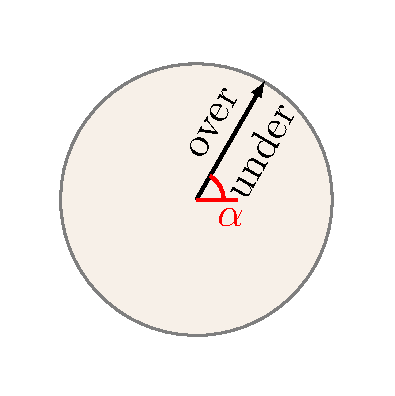
\includegraphics[width=0.17\textwidth]{../assets/840/over_under_2.pdf}}
%
and each point $p$ on a strand $S$ satisfying $\Arg(S,p)=\alpha$ is marked by $\mysq$ as in \cref{fig:over_under}.
\end{remark}






\section{Positroid link isotopies}\label{sec:positr-link-isot}
The goal of this section is to prove \cref{thm:isotopy}. We first discuss some properties of plabic graph links, and then we construct a sequence of isotopies, for any permutation $\pi\in\Sn$ without fixed points, of the links
\begin{equation*}%
\Lrich_\pi \cong  \Lplab_\pi \cong \Lperm_\pi \cong \Ltor_\pi,
\end{equation*}
in that order. When $\pi=\pi_C$ for some concave curve $C$, we will also show that
\begin{equation*}%
  \Ltor_\pi\cong\Lcox_\pi,
\end{equation*}
completing the proof.

%
%

Throughout this section, we fix a permutation $\pi\in\Sn$ without fixed points, and let $(v,w)\in\Qkn$ be the corresponding pair satisfying $\pi=wv^{-1}$,  $\Gamma$ the corresponding Le-diagram of shape $\la$, and $G$ the corresponding plabic graph, obtained from $\Gamma$ using the recipe in the first two rows of \cref{fig:Le_to_G}.

\subsection{From Richardson links to plabic graph links}\label{sec:from-rich-links}
 Our goal is to construct an isotopy between the Richardson link $\Lrich_{v,w}$ (\figref{fig:Lrich}(right)) and the plabic graph link $\Lplab_G$ (\figref{fig:Lplab}(c)).

Recall from \cref{rmk:Rich_Young} that we are drawing the Richardson braid $\beta_{v,w}=\beta(w)\cdot \beta(v)^{-1}$ in a particular way, so that the crossings of $\beta(w)$ form a shape obtained by rotating $\la$ clockwise by $135^\circ$, and the crossings of $\beta(v)^{-1}$ are drawn in some boxes of a shape obtained from the $135^\circ$-rotation of $\la$ by reflecting it along the vertical axis; see \figref{fig:Lrich}(left). Moreover, the crossings of $\beta(v)^{-1}$ are located precisely in the boxes of $\la$ which do not contain a dot in $\Gamma$. 
 %

\begin{figure}
  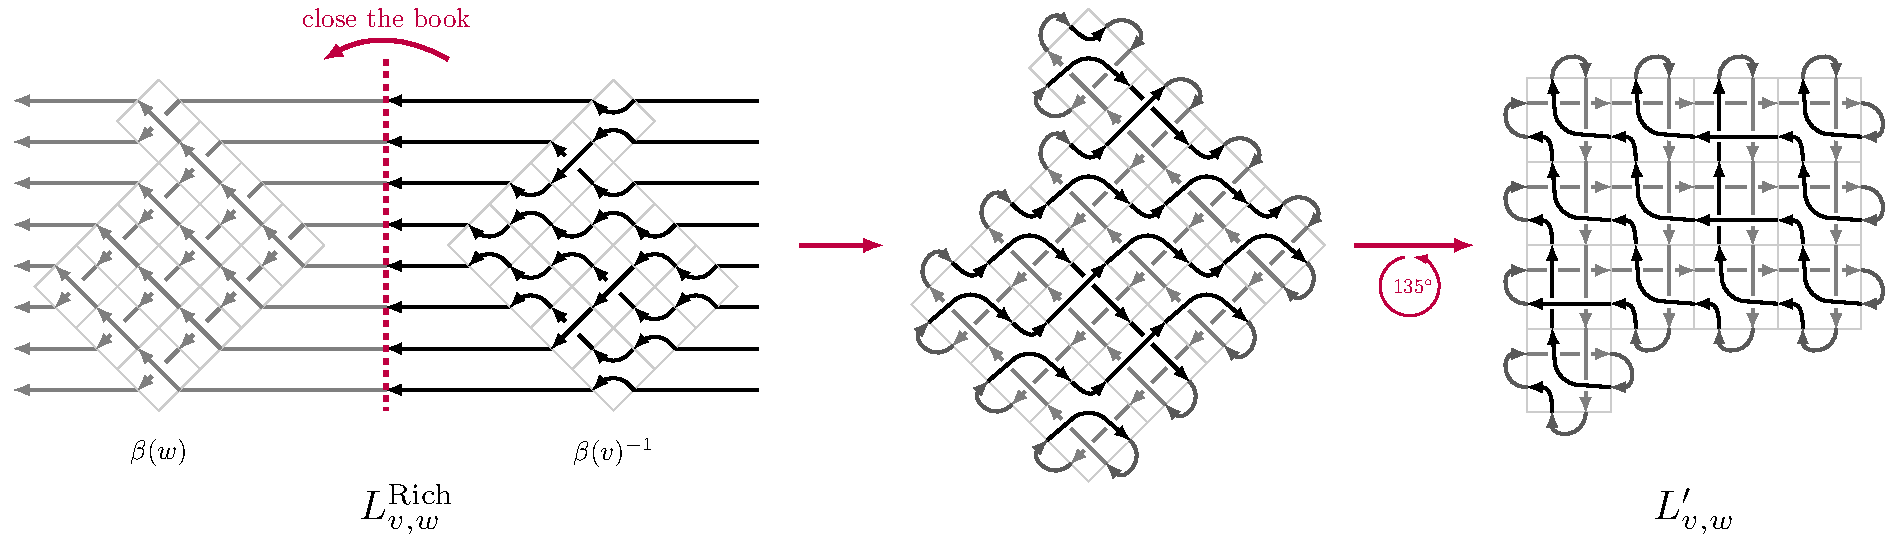
\includegraphics[width=1.0\textwidth]{../assets/840/Lrich_to_Lprime.pdf}
  \caption{\label{fig:Lrich-to-L'} Converting the link $\Lrich_{v,w}$ into $\Lrichp_{v,w}'$; see \cref{sec:from-rich-links}.}
\end{figure}


Our first goal is to draw the link $\Lrich_{v,w}$ entirely within $\la$. To do that, we take $\beta(v)^{-1}$, reflect it along the vertical axis (flipping the over/under-crossings), and place the resulting braid on top of $\beta(w)$. We rotate the result counterclockwise by $135^\circ$. Every line segment in the boundary of $\la$ contains an endpoint of a strand in $\beta(v)^{-1}$ and an endpoint of a strand in $\beta(w)$. We join these strand endpoints, obtaining a link diagram drawn inside of $\la$. This link $\Lrichp_{v,w}'$, shown in \cref{fig:Lrich-to-L'}, is clearly isotopic to $\Lrichp_{v,w}$. Intuitively, the transformation $\Lrich_{v,w}\to\Lrichp_{v,w}'$ can be described as follows: open a book, and place the left (resp. right) half of \figref{fig:Lrich}(right) onto the left (resp. right) page of the book. Then close the book with your right hand, so that the front cover of the book is at the bottom. The page containing (the reflection of) $\beta(v)^{-1}$ will be on top of the page containing $\beta(w)$. Finally, rotate the closed book $135^\circ$ counterclockwise. 


\begin{figure}
  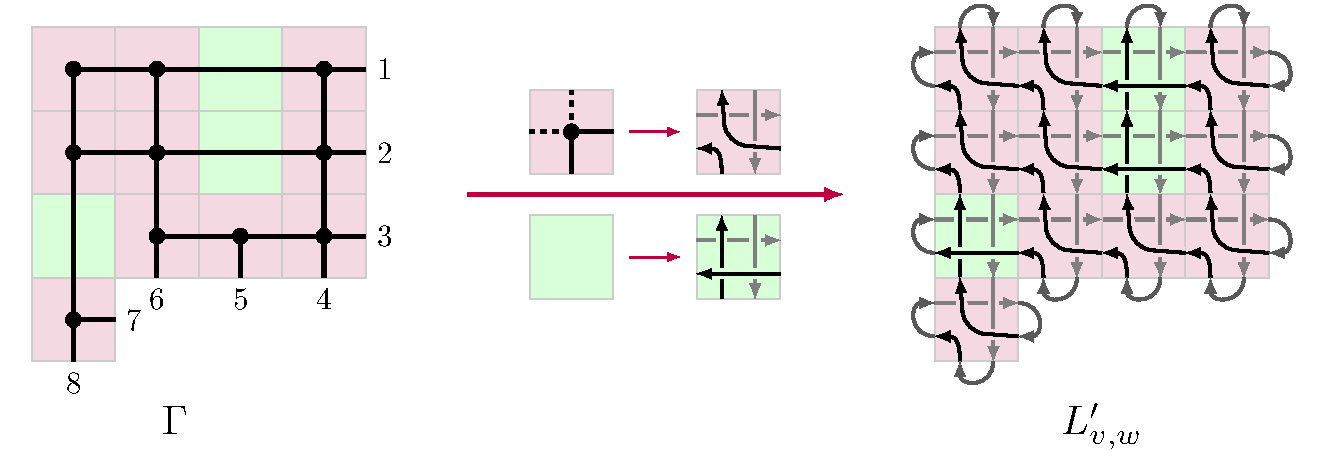
\includegraphics[width=0.9\textwidth]{../assets/840/Gamma_to_Lprime.pdf}
  \caption{\label{fig:Gamma-to-L'} Converting a Le-diagram $\Gamma$ into a link $L'_{v,w}$.}
\end{figure}




An alternative description of the link $\Lrichp_{v,w}'$ can be obtained directly from the Le-diagram $\Gamma$ by replacing each box containing a dot as shown in \figref{fig:Gamma-to-L'}(middle top) and each box not containing a dot as shown in \figref{fig:Gamma-to-L'}(middle bottom). For example, the Le-diagram in \figref{fig:Gamma-to-L'}(left) gets converted into the link $\Lrichp_{v,w}'$ in \figref{fig:Gamma-to-L'}(right); this is the same link as in \figref{fig:Lrich-to-L'}(right). Since $\pi$ has no fixed points, each row and each column of $\Gamma$ contains at least one dot. Consider some column $j$ of $\Gamma$ and let $b_j$ be the highest box in it which contains a dot. The part of $\Lrichp_{v,w}'$ above $b_j$ contains a strand going vertically to the top boundary and then back, passing between all the horizontal strands that it encounters along the way. We may therefore contract this piece of the strand to be fully contained inside $b_j$, as shown in \figref{fig:pull}(far left). Repeating this procedure for each column $j=1,2,\dots,\la_1$, we obtain a link $\Lrichp_{v,w}''$ isotopic to $\Lrichp_{v,w}'$; see \figref{fig:pull}(middle).

\begin{figure}
  \setlength{\tabcolsep}{0pt}
\begin{tabular}{c|c}
\begin{tikzpicture}[baseline=(Z.base)]
\coordinate(Z) at (0,0);
\node(A) at (0,2.05){
  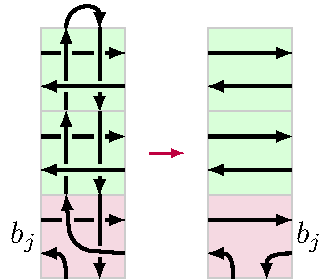
\includegraphics[width=0.2\textwidth]{../assets/840/pull.pdf}
};
\end{tikzpicture}
&
  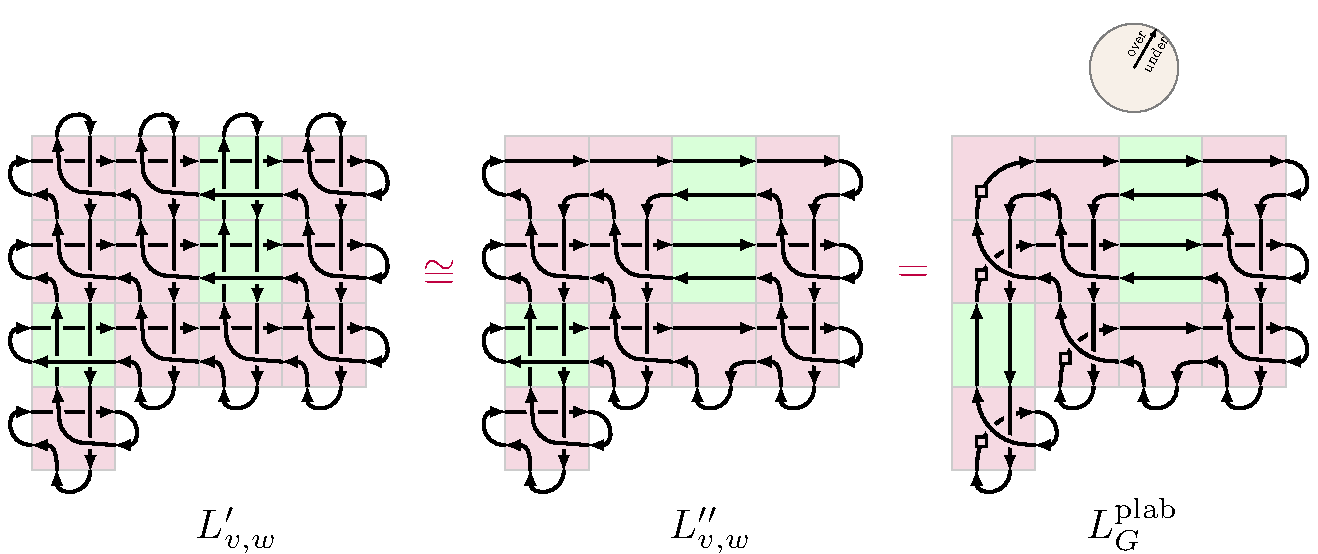
\includegraphics[width=0.78\textwidth]{../assets/840/pull_to_L.pdf}
\end{tabular}
  \caption{\label{fig:pull} An isotopy from $\Lrichp_{v,w}'$ to $\Lplab_G$.}
\end{figure}



Finally, we claim that the link $\Lrichp_{v,w}''$ is isotopic to the plabic graph link $\Lplab_G$. To see this, we choose the angle $\alpha$ from \cref{rmk:rotation} to be $80^\circ$. Then combining the rules from \cref{fig:Le_to_G} for converting the Le-diagram $\Gamma$ into the plabic graph $G$ with the description of $\Lplab_G$ given in \cref{sec:plabic_links_properties}, we see that a planar diagram of $\Lplab_G$ is obtained from $\Gamma$ via the rules shown in the last two rows of \cref{fig:Le_to_G}. Replacing each square (where $\Arg(S,p)=\alpha$) by a horizontal segment going to the left boundary above all other strands and back below all other strands, we see that $\Lplab_G= \Lrichp_{v,w}''$; see \figref{fig:pull}(far right). To summarize, we have constructed explicit isotopies
\begin{equation*}%
  \Lrich_\pi=\Lrich_{v,w}\cong\Lrichp_{v,w}'\cong\Lrichp_{v,w}''=\Lplab_G.
\end{equation*}



\begin{figure}
  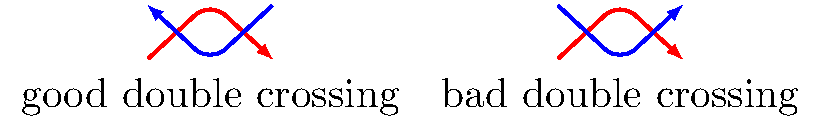
\includegraphics[width=0.5\textwidth]{../assets/840/double.pdf}
  \caption{\label{fig:double} Good and bad double crossings of strands in plabic graphs.}
\end{figure}


\subsection{From plabic graph links to permutation links}
Our goal is to find an isotopy $\Lplab_\pi\cong \Lperm_\pi$. Let $G$ be a reduced plabic graph with strand permutation $\pi$. Let $\Divide=\Divide(G)$ be the oriented divide obtained from $G$ as in \cref{sec:plabic_links_properties}. Let $1,2,\dots,\n$ be the boundary vertices of $G$. Since $G$ is reduced, it contains no bad double crossings shown in \figref{fig:double}(right). Thus, it is clear that applying the moves from \cref{fig:divide_moves}, one can transform $\Divide$ into an oriented divide $\Divide'$ obtained by drawing a straight arrow $i\to \pi(i)$ for each $i\in[\n]$. The moves from \cref{fig:divide_moves} give rise to link isotopies, so $L_\Divide\cong L_{\Divide'}$. Let us move the boundary vertices $1,2,\dots,\n$ smoothly to the points $1',2',\dots,\n'$ which are located clockwise on the left semicircle of $\partial \disk$, i.e.  on the subset of $\partial\disk$ with negative real part. Let $\Divide''$ be the oriented divide obtained by drawing a straight arrow $i'\to \pi(i)'$ for each $i\in[\n]$. It follows that $L_{\Divide'}\cong L_{\Divide''}$.
%
 Let $i,j\in[\n]$ be such that the corresponding arrows $S_i:=(i'\to \pi(i)')$ and $S_j:=(j'\to \pi(j)')$ of $\Divide''$ cross at some point $p$. Consider the arguments of the tangent vectors $0\leq \Arg(S_i,p)\neq\Arg(S_j,p)<2\pi$. Then it is easy to check that $\Arg(S_i,p)>\Arg(S_j,p)$ if and only if $\pi(i)<\pi(j)$. 
%
 Comparing to the description in \cref{sec:intro:perm_links}, we get that $L_{\Divide''}\cong\Lperm_\pi$.



\subsection{From permutation links to toric permutation links}\label{sec:perm-to-toric}
Our goal is to find an isotopy $\Lperm_\pi\cong\Ltor_\pi$. Recall from \cref{rmk:grid} that $\Ltor_\pi$ is isotopic to the \emph{planar grid link} denoted $\Lgrid_\pi$; see \figref{fig:grid_iso}(a--c). In $\Lgridt_\pi$ and $\Lgrid_\pi$, the vertical arrows are drawn above the horizontal arrows. 

The main diagonal $y=1-x$ of the square $[0,1]^2$ divides $\Lgrid_\pi$ into the \emph{lower-triangular} and the \emph{upper-triangular} parts. In the lower-triangular part, all vertical arrows point down and all horizontal arrows point right, while in the upper-triangular part, all vertical arrows point up and all horizontal arrows point left. 
Let us take the lower-triangular part and reflect it around the main diagonal, placing it below the upper-triangular part; see \figref{fig:grid_iso}(c--d). We obtain a planar diagram of a link which we denote $L_\pi'$. Clearly, $L_\pi'\cong \Lgrid_\pi$. The diagram of $L_\pi'$ contains arrows pointing, up, left, down, and right. It follows that the over/under-crossings rule  in $L_\pi'$ is given by the following total order on the arrow directions: up $>$ left $>$ down $>$ right. In particular, $L_\pi'$ is a divide link for the angle $\alpha=45^\circ$ from \cref{rmk:rotation} (where the main diagonal is treated as part of the boundary of the disk), and we get that $L_\pi'\cong\Lperm_\pi$. 
%

\subsection{From toric permutation links to Coxeter links}\label{sec:tor_to_Cox}
First, we introduce a more general class of links, associated to arbitrary monotone curves inside the $k\times(\n-k)$ rectangle.

%
%
We say that $C_g$ is a \emph{monotone curve} if it is the plot of a strictly monotone increasing function $g(x):[0,\n-k]\to[0,k]$ satisfying $g(0)=0$, $g(\n-k)=k$, and $g(j)\notin\Z$ for all $j=1,2,\dots,\n-k-1$. Thus, the curve $C_g$ passes through the points $(0,0)$ and $(\n-k,k)$, but through no other lattice points. To any monotone curve $C_g$ we associate a link $L_g$ drawn on the surface of $\T$. The planar diagram of $L_g$ is obtained from the projection $\Cproj_g$ of $C_g$ to $\T$ via the following rule: whenever  two points $(x,g(x))$, $(x',g(x'))$ on $C_g$ (with $x<x'$) project to the same point of $\Cproj_g$, we draw the projection of $(x,g(x))$ above the projection of $(x',g(x'))$. 

The link diagram of $L_g$ is drawn on the torus $\T$, and therefore it is natural to think of $L_g$ itself as a link inside the \emph{thickened torus} $\T\times[0,1]$. Given a point $p=(x,g(x))\in C_g$, we denote by $\projtx p\in \T$ the projection of $p$ to $\T$, and we let $\left(\projtx p,1-\frac{x}{\n-k}\right)$ be the corresponding point in $\T\times[0,1]$. This yields an embedding of $C_g$ into $\T\times[0,1]$. Under this embedding, the points $(0,0)$ and $(\n-k,k)$ map to $((0,0),1)$ and $((0,0),0)$, respectively. Adding a line segment connecting $((0,0),1)$ to $((0,0),0)$, we obtain a representation of the link $L_g$ inside $\T\times[0,1]$. An obvious consequence of this construction is that the link $L_g$ only depends on the set of lattice points below the plot of $g$.
\begin{corollary} \label{cor:monotone_curves}
Let $C_g$, $C_h$ be two monotone curves, and assume that for each $j=1,2,\dots,\n-k-1$, we have $\lfloor g(j)\rfloor=\lfloor h(j)\rfloor$. Then the links $L_g$ and $L_h$ are isotopic. 
\end{corollary}

Suppose now that $\pi=\pi_C$ for a concave curve $C$. Our goal is to find an isotopy $\Ltor_\pi\cong\Lcox_C$. Comparing the above description to the one in \cref{sec:intro:cox_link}, we see that when $g$ is the concave down function satisfying $C=C_g$, we have $\Ltor_\pi\cong L_g$. Our goal is to choose a monotone curve $C_h$ such that $L_g\cong L_h$ by \cref{cor:monotone_curves}, and such that $L_h\cong \Lcox_C$. 
 %

\begin{figure}
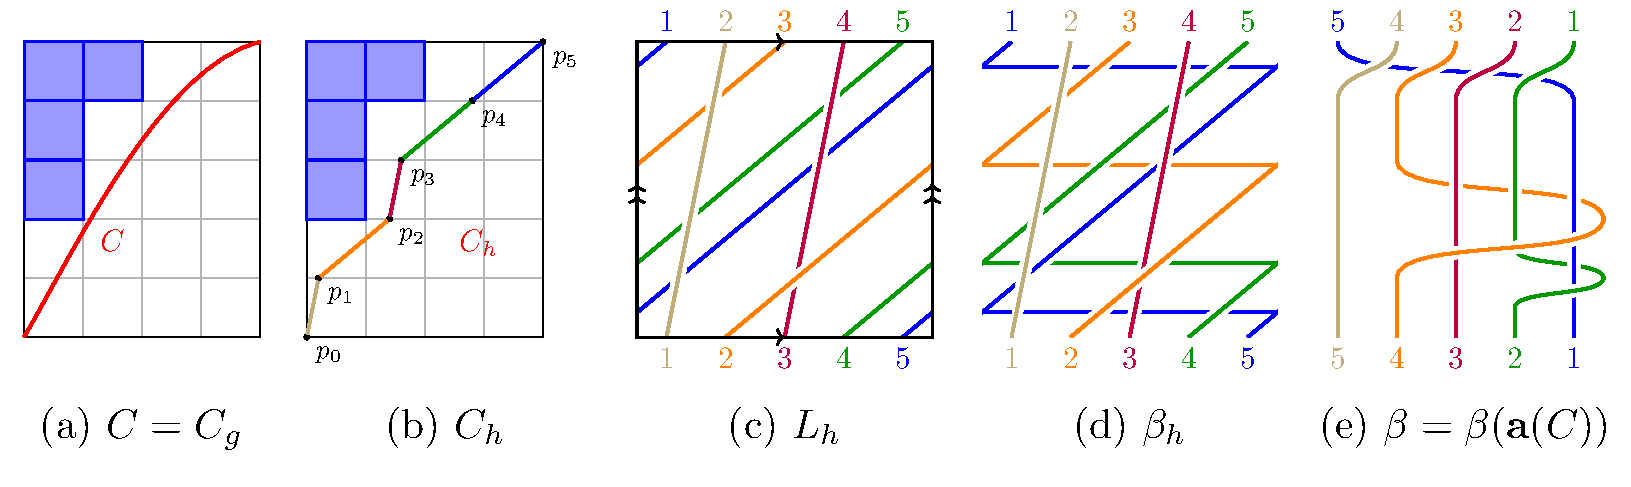
\includegraphics[width=1.0\textwidth]{../assets/840/C_to_beta.pdf}
  \caption{\label{fig:C_to_beta} Converting a concave curve $C$ into the Coxeter link $\beta(\abf(C))$; see \cref{sec:tor_to_Cox}.}
\end{figure}


Let $\la=\la_C=(\la_1\geq \la_2\geq\dots\geq \la_k=0)$ be the Young diagram above $C$. For $r=0,1,\dots,k-1$, let $p_r:= \left(\la_{k-r}+\frac rk,r\right)$. Thus, $p_0=(0,0)$. Let $p_{k}:=(\n-k,k)$. Let $h$ be the piecewise-linear function whose plot passes through the points $p_0,p_1,\dots,p_k$, and let $C_h$ be the corresponding monotone curve; see \figref{fig:C_to_beta}(b). Indeed, by \cref{cor:monotone_curves}, we have $L_g\cong L_h$. It remains to establish the isotopy $L_h\cong \Lcox_C$. 

Let $\beta=\beta(\abf(C))$ be the Coxeter braid associated to $C$, defined in~\eqref{eq:beta_abf_dfn}. It is a braid on $k$ strands. For $i=1,2,\dots,k$, let $S_i(\beta)$ be the strand of $\beta$ whose left endpoint is labeled by~$i$. Thus, the right endpoint of $S_i(\beta)$ is labeled by $i+1$ for $i<k$ and by $1$ for $i=k$. On the other hand, the link diagram of $L_h$ in $\T$ intersects the line $y=0$ in exactly $k$ points with horizontal coordinates $\frac rk$ for $r=0,1,\dots, k-1$. We would like to view $L_h$ as the closure of a $k$-strand braid $\beta_h$ in the solid torus; see \figref{fig:C_to_beta}(c--d). The braid $\beta_h$ is obtained from $L_h$ via the following procedure: whenever a strand of $L_h$ passes through some point $(1,y)\in[0,1]^2$ and continues from the point $(0,y)\in[0,1]^2$, we connect the points $(0,y)$ and $(1,y)$ by a horizontal line segment that is drawn below all strands of $L_h$. The result is a drawing of a braid connecting $k$ points at the bottom of $[0,1]^2$ to $k$ points at the top of $[0,1]^2$. 

For $i=1,2,\dots, k-1$, let $S_i(\beta_h)$ be the piece of $\beta_h$ connecting the point $(\frac{i-1}k,0)$ to the point $(\frac ik,1)$. For $i=k$, let $S_k(\beta_h)$ be the remaining piece of $\beta_h$, connecting $(\frac{k-1}k,0)$ to $(0,1)$. See \figref{fig:C_to_beta}(d--e).

We claim that the braids $\beta_h$ and $\beta$ are isotopic. We compare them strand-by-strand, identifying $S_i(\beta)$ with $S_{k+1-i}(\beta_h)$ for $i=1,2,\dots,k$, in that order. (This correspondence is indicated via colors in \figref{fig:C_to_beta}(d--e).) For convenience, we rotate the drawing of $\beta$ by $90^\circ$ counterclockwise. The strand $S_1(\beta)$ moves straight up during the $\ell_2^{a_2}\cdots \ell_k^{a_k}$ part, and then it moves left under all other strands. We apply an isotopy to make $S_k(\beta_h)$ move straight up towards the top boundary of $[0,1]^2$, and then move left under all other strands. Recall that we have a sequence $\abf(C)=(a_2,\dots,a_k)$ given by $a_i=\la_{i-1}-\la_i$ for $i=2,\dots,k$. Thus, the strand $S_2(\beta)$ wraps around $S_1(\beta)$ exactly $a_2$ times. On the other hand, $S_{k-1}(\beta_h)$ is the projection to $\T$ of the line segment of $C_h$ connecting $p_{k-1}$ to $p_k$. This projection intersects the vertical boundary of $\T$ exactly $a_2$ times. Therefore $S_{k-1}(\beta_h)$ wraps around $S_k(\beta_h)$ exactly $a_2$ times. Continuing in this fashion, we see that for $i=3,\dots,k$, the strand $S_i(\beta)$ wraps around the union $S_1(\beta)\cup S_2(\beta)\cup\dots\cup S_{i-1}(\beta)$ exactly $a_i$ times. On the other hand, the strand $S_{k+1-i}(\beta_h)$ wraps around the union $S_k(\beta_h)\cup S_{k-1}(\beta)\cup\dots\cup S_{k+2-i}$ exactly $a_i$ times. This shows that the braids $\beta$ and $\beta_h$ are isotopic, and therefore we get an isotopy $\Lcox_C\cong L_h$ between their closures.

\begin{remark}
The above construction is extended to links with multiple components (resp. to monotone curves passing through some lattice points in the interior of the rectangle) in~\cite[Section~7.3]{GL_EHA}.
\end{remark} 


\section{Quivers}
In this section, we introduce the point count polynomial $R(Q;q)$ of a \Louise %
 quiver, and study its basic properties.  We use this polynomial to define the \emph{$Q$-Catalan number} of $Q$, an integer that we conjecture to be nonnegative in \cref{conj:Catalan}. We refer the reader to~\cite{FWZ_book} for an excellent introduction to quivers and cluster algebras.

\subsection{Quiver mutation}\label{sec:quiver}
Recall that a \emph{quiver} is a directed graph without directed cycles of length $1$ and $2$.

Given a quiver $Q$ and a vertex $j\in V(Q)$, one can define another quiver $Q'=\mu_j(Q)$ called the \emph{mutation of $Q$ at $j$}. This operation preserves the set of vertices:  $V(Q')=V(Q)$, and changes the set of arrows as follows:
\begin{itemize}
\item for every length $2$ directed path $i\to j\to k$ in $Q$, add an arrow $i\to k$ to $Q'$;
\item reverse all arrows in $Q$ incident to $j$;
\item remove pairs of opposite arrows (i.e.  directed $2$-cycles) in the resulting directed graph, one pair at a time, until no such pairs are present.
\end{itemize}

An \emph{ice quiver} is a quiver $\Qice$ whose vertex set $\Vice=V(\Qice)$ is partitioned into \emph{frozen} and \emph{mutable} vertices: $\Vice=\Vfro\sqcup \Vmut$. We automatically omit all arrows in $\Qice$ both of whose endpoints are frozen. For an ice quiver $\Qice$, its \emph{mutable part} is the induced subquiver of $\Qice$ with vertex set $\Vmut$.  %
 For a set $S\subset \Vmut$, let $\Qicefr[S]$ denote the ice quiver obtained from $\Qice$ by further declaring all vertices in $S$ to be frozen. We write $\Qice-S$ for the ice quiver obtained from $\Qice$ by removing the vertices in $S$.  For a simply-laced Dynkin diagram $D$, we say that $Q$ or $\Qice$ has type $D$, or is a $D$-quiver, if the underlying graph of $Q$ is isomorphic to $D$.


 Let $\Qice$ be an ice quiver with $\Vice=[n+m]$, $\Vmut=[n]$, and $\Vfro=[n+1,n+m]:=\{n+1,n+2,\dots,n+m\}$. We represent it by an $(n+m)\times n$ \emph{exchange matrix} $\BQice=(b_{ij})$, defined by
 \begin{equation*}%
   b_{ij}=\#\{\text{arrows $i\to j$ in $\Qice$}\} - \#\{\text{arrows $j\to i$ in $\Qice$}\}.
 \end{equation*}
The top $n\times n$ submatrix $\BQ$ of $\BQice$ is skew-symmetric, and is called the \emph{principal part} of $\BQice$.  
%

%
%
%
%
%
%
%
%
%
%
%
%
%
%
%
%
 
%

Let $\Bice$ be an $(n+m)\times n$ matrix. We denote $\cork(\Bice):=n-\rk(\Bice)$. Following~\cite{LS}, we say that an $(n+m)\times n$ matrix $\Bice$ is \emph{really full rank} if the rows of $\Bice$ span $\Z^n$ over $\Z$. We say that $\Qice$ is \emph{really full rank} if $\BQice$ is really full rank, and write $\cork(\Qice):=\cork(\BQice)$.   We say that $\Qice$ is \emph{torsion-free} if the abelian group $\Z^{n+m}/\BQice \Z^n$ is torsion-free, equivalently, if $\Z^n/\BQice^T \Z^{n+m}$ is torsion-free.  Thus, $\Qice$ is really full rank if and only if it is both full rank and torsion-free.

\begin{definition}
Given a quiver $Q$, we say that an ice quiver $\Qice$ with mutable part $Q$ is a \emph{minimal extension} of $Q$ if $\Qice$ has $m=\cork(Q)$ frozen vertices and is really full rank.
\end{definition}

\begin{lemma}\label{lem:ext}
If $Q$ is torsion-free then it admits a minimal extension.
%
\end{lemma}
\begin{proof}
If $Q$ is torsion-free, we can find vectors $d_1,\ldots,d_m \in \Z^n$ that form a basis of $\Z^n/B(Q)^T \Z^n$.  Define $\Qice$ with $m$ frozen vertices so that the bottom $m$ rows of the exchange matrix $\Bice$ are equal to $d_1,\ldots,d_m$.
\end{proof}
%
%

\begin{example}
The exchange matrices of the two quivers $Q,Q'$ in \figref{fig:LA}(c) are given by
$$
\BQ=\begin{pmatrix}
0 & 2 & -2 \\
-2&0&2\\
2&-2&0
\end{pmatrix} \qquad \text{and} \qquad
B(Q')=\begin{pmatrix}
0 & -1& -1 &2 \\
1&0&1 &-1\\
1&-1&0 &-1 \\
-2&1&1&0
\end{pmatrix}.
$$
Thus, $\cork(Q)=1$, $\cork(Q')=0$, and neither quiver is torsion-free.
\end{example}

We say that an ice quiver $\Qice$ is \emph{isolated} if it has no arrows. For example, the quiver in \figref{fig:simple}(c) is isolated.

We call an ice quiver $\Qice$ \emph{acyclic} if it has no directed cycles, and \emph{mutation acyclic} if it is mutation equivalent to an acyclic ice quiver.  For example, any quiver of Dynkin type is acyclic, as is the quiver in \figref{fig:LA}(a).  The quiver in \figref{fig:simple}(a) and the left quiver in \figref{fig:LA}(b) are not acyclic, but they are both mutation acyclic, since mutating a single vertex in each of these quivers makes them acyclic.

An edge $u\to v$ in a quiver $Q$ is called a \emph{separating edge}~\cite{Muller} if it does not belong to a bi-infinite walk in $Q$. Here, a \emph{bi-infinite walk} is a sequence $(w_j)_{j\in\Z}$ of vertices in $Q$ such that for each $j\in\Z$, $Q$ contains an arrow $w_j\to w_{j+1}$.

We define the class of \emph{\Louise quivers}, called ``Louise" in \cite{MSLA,LS}, as follows.
\begin{itemize}
\item Any isolated quiver $Q$ is \Louise.
\item Any quiver that is mutation equivalent to a \Louise quiver is \Louise.
\item Suppose that a quiver $Q$ has a separating edge $u\to v$, and that all three quivers $Q-\{u\}$, $Q-\{v\}$, $Q-\{u,v\}$ are \Louise. Then $Q$ is \Louise.
\end{itemize}
We say that an ice quiver $\Qice$ is \emph{\Louise} if its mutable part $Q$ is \Louise.    See \cref{fig:LA}.
\begin{figure}
  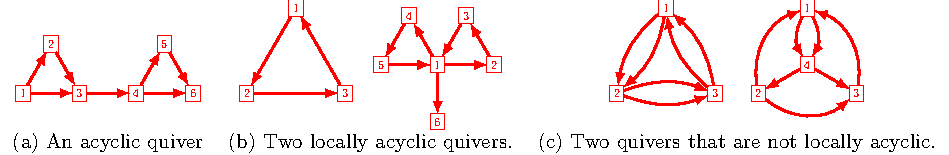
\includegraphics[width=\textwidth]{../assets/840/Louise.pdf}
  \caption{\label{fig:LA} Acyclic, locally acyclic and non-\Louise quivers.}
\end{figure}

\subsection{Cluster algebras}
Let $\Qice$ be an ice quiver with $\Vice=[n+m]$, $\Vmut=[n]$, and $\Vfro=[n+1,n+m]$.  We associate to $\Qice$ the initial seed $(x_1,x_2,\ldots,x_{n+m})$ of \emph{cluster variables}, considered as elements in the function field $\Fcal = \Q(x_1,x_2,\dots,x_{n+m})$.  The variables $x_{n+1},\ldots,x_{n+m}$ are called \emph{frozen variables}.  For a mutation $Q' = \mu_j(Q)$, we associate the seed $(x'_1,x'_2,\ldots,x'_{n+m})$, where $x'_i = x_i$ if $i \neq j$ and one has the new cluster variable
$$
x'_j = \frac{\prod_{r \to j} x_r + \prod_{j \to s} x_s}{x_j} \in \Fcal.
$$
By repeatedly mutating, we generate (possibly infinitely) many seeds and cluster variables. 
 We denote by $\AQice=\ABQice$ the cluster algebra associated to $\Qice$. This is the $\Z$-subalgebra of $\Q(x_1,x_2,\dots,x_{n+m})$ generated by all cluster variables and the inverses of frozen variables. 
 
The \emph{cluster variety} $\XQice=\XBQice$ is defined to be the scheme
\begin{equation*}%
\XQice:=\Spec(\AQice).
\end{equation*}
We say that $\AQice$ (resp. $\XQice$) is a cluster algebra (resp. cluster variety) \emph{of type $Q$}, where $Q$ is the mutable part of $\Qice$.  We say that $\AQice$ is isolated, acyclic, (really) full rank, if $\Qice$ is isolated, mutation acyclic, (really) full rank, respectively.  If $\Qice$ is a \Louise quiver, then $\AQice$ is locally acyclic in the sense of Muller~\cite{Muller}.


\begin{proposition}[{\cite[Theorem 7.7]{Muller}, \cite[Theorem 10.1]{LS}}]\label{prop:Mulsmooth}
Suppose that $\Qice$ is \Louise and really full rank.  Then $\XQice_\C$ is a smooth complex algebraic variety and $\XQice_{\bar \F_q}$ is smooth for any prime power $q$.
\end{proposition}

\begin{proposition}[{\cite[Corollary 5.4]{Muller}}]\label{prop:Mulcover}
Let $i \to j$ be a separating edge in $\Qice$.  Then the open sets $\{x_i \neq 0\}$ and $\{x_j \neq 0\}$ cover $\XQice$.
\end{proposition}

\begin{proposition}[{\cite[Proposition 3.1, Lemma 3.4, Theorem 4.1]{Muller}}]\label{prop:Mulloc}
Suppose that $i \in V(\Qice)$ is a mutable vertex such that $Q- \{i\}$ is \Louise.  Then $\AQice[x_i^{-1}] \simeq \AX(\Qice[i])$.
\end{proposition}

\subsection{Quiver point count}
For a mutable quiver $Q$, we define the function $\RQ(q)$ as follows. Choose a really full rank ice quiver $\Qice$ with mutable part $Q$ and $m$ frozen vertices. Then for $q$ a prime power, we set
\begin{equation}\label{eq:RQ_dfn}
  \RQ(q):=\frac{\#\XQice(\F_q)}{(q-1)^m}.
\end{equation}
For a rational function $R(q)=P(q)/Q(q)$, we let the \emph{degree} $\deg(R)$ be the difference $\deg(P)-\deg(Q)$. 
\begin{proposition}[{\cite[Proposition 5.11 and Theorem 10.5]{LS}}]\label{prop:Q_pcnt}
  Let $Q$ be a quiver with $n$ vertices.
  \begin{enumerate}
  \item The function $\RQ(q)$ defined in~\eqref{eq:RQ_dfn} does not depend on the choice of $\Qice$.
  \item Suppose $Q$ is \Louise. Then $\RQ(q)$ is a rational function in $q$ of degree $n$. %
  \end{enumerate}
\end{proposition}
If $u \to v$ is a separating edge in $Q$ and $Q-\{u\},Q-\{v\},Q-\{u,v\}$ are \Louise, then we have the recurrence
\begin{equation}\label{eq:RQ_recurrence}
  \RQ(q) = (q-1)\RQX{Q-\{u\}}{q}+ (q-1)\RQX{Q-\{v\}}{q}- (q-1)^2\RQX{Q-\{u,v\}}{q},
\end{equation}
which follows from Propositions~\ref{prop:Mulcover} and~\ref{prop:Mulloc}.

\begin{proposition}[{\cite[Proposition 3.9]{LS2}}] \label{prop:acycliccount}
Let $Q$ be an acyclic quiver with $n$ vertices.  Then 
$$
\RQ(q) = \sum_{k \geq 0} a_k (q-1)^{n-2k} q^k,
$$
where $a_k$ is the number of independent sets of size $k$ in the underlying undirected graph of~$Q$.
\end{proposition}

When $Q$ itself is really full rank, $\RQ(q)$ is a polynomial in $q$. However, $\RQ(q)$ is in general a genuine rational function whose denominator is a power of $(q-1)$. For example, for $Q$ a single isolated vertex (we denote this quiver by $A_1$; it has corank $1$), we have
\begin{equation}\label{eq:A1}
  \RQX{A_1}{q}=\frac{q^2-q+1}{q-1}.
\end{equation}
For an ice quiver $\Qice$ with mutable part $Q$ and $m$ frozen vertices, we set
\begin{equation*}%
  \RQice(q):=(q-1)^m\RQ(q).
\end{equation*}
Thus, when $\Qice$ is really full rank and \Louise, $\RQice(q)$ is a polynomial in $q$ of degree $n+m$ satisfying $\#\XQice(\F_q)=\RQice(q)$ for all prime powers $q$.
\begin{definition}\label{def:QCat}
Let $Q$ be a torsion-free quiver, and $\Qice$ be a minimal extension as in \cref{lem:ext}.  If $\RQice(q)$ is a polynomial in $q$, define %
  \begin{equation*}%
    \chiQ:=\RQice(1).
  \end{equation*}
  By \cref{prop:Q_pcnt}, $\chiQ$ does not depend on the choice of $\Qice$.
\end{definition}
We call $\chiQ$ the \emph{Catalan number} of the quiver $Q$, or simply the \emph{$Q$-Catalan number}.

\begin{conjecture}\label{conj:Catalan}
Suppose that $Q$ is a \Louise quiver. %
Then $\chiQ \geq0$. %
\end{conjecture}
%

We note that $\chiQ$ can be zero.  For example, let $Q$ be an acyclic orientation of the three-cycle, and let $\Qice$ be a minimal extension. Thus, $\Qice$ is a really full rank quiver with $\cork(Q)=1$ frozen vertices.
%
 Then by \cref{prop:acycliccount}, we have $R(Q;q)=(q-1)^3+3(q-1)q$, and thus $R(\Qice;q) = (q-1)^4+3(q-1)^2q$ and  $\chiQ =0$.  For another example, the quiver $Q$ in \figref{fig:LA}(a) satisfies $\cork(Q) = 0$ and $\chiQ = 0$.  %

Consider a polynomial $R(q)$ of degree $n$ with integer coefficients  that is palindromic (i.e.  satisfies $q^nR(1/q)=R(q)$). One can show by induction that it can be written as $\sum_{k=0}^{\lfloor n/2\rfloor} a_k (q-1)^{n-2k} q^k$ for unique coefficients $a_0,a_1,\dots,a_{\lfloor n/2\rfloor}\in\Z$. It follows from the \emph{curious Lefschetz property} shown in~\cite{LS} that the point count polynomial of any \Louise really full rank quiver is palindromic. We thank the anonymous referee for suggesting the first part of the following strengthening of \cref{conj:Catalan}. 
\begin{conjecture}
Let $Q$ be a \Louise quiver, and let $\Qice$ be a really full rank quiver with $n$ vertices and mutable part $Q$. Then we have 
\begin{equation*}%\label{eq:*}
  \RQice(q) = \sum_{k=0}^{\lfloor n/2\rfloor} a_k (q-1)^{n-2k} q^k, \quad\text{where each $a_k \geq0$.}
\end{equation*}
Moreover, the cluster variety $\XQice$ over a field $\F$ may be represented as a disjoint union over $0\leq k\leq\lfloor n/2\rfloor$ of $a_k$ copies of $(\F^\ast)^{n-2k} \times\F^k$.
\end{conjecture}
\setcounter{theo}{13}\setcounter{equation}{4}
\subsection{Leaf recurrence}
%
Let $i\in V(Q)$ be a leaf vertex of a quiver $Q$, connected to some other vertex $j\in V(Q)$. We call $i$ a \emph{\Louiseleaf} if both quivers $Q-\{i\}$ and $Q-\{i,j\}$ are \Louise.  This automatically implies that $Q$ itself is \Louise.

%

\begin{proposition}\label{prop:Louise_leaf}
Fix a field $\Ga$, and consider cluster varieties over $\Ga$.
Let $\Qice$ be a really full rank ice quiver with $m$ frozen vertices and mutable part $Q$. Let $i\in V(Q)$ be a \Louiseleaf in $Q$ connected to $j\in V(Q)$. Then the subvariety of $\XQice$ given by $x_i=0$ is isomorphic to $\Ga\times \Xcal(\Qice')$, where $\Qice'$ is a really full rank quiver with $m$ frozen vertices and mutable part $Q':=Q-\{i,j\}$.
\end{proposition}
\begin{proof}%
Our goal is to construct a quiver $\Qice'$ satisfying the above assumptions and an isomorphism
\begin{equation}\label{eq:leaf1}
  \{\bx\in\Xcal(\Qice)\mid x_i=0\} \cong \F\times \Xcal(Q').
\end{equation}

  By Proposition~\ref{prop:Mulcover}, the subvariety of $\Xcal(\Qice)$ given by $x_i=0$ is contained inside the subvariety of $\XQice$ given by $x_j\neq0$. The quiver $Q-\{j\}$ is the disjoint union of $Q'$ and a single isolated vertex. By assumption, $Q'$ is \Louise and thus so is $Q-\{j\}$. By Proposition~\ref{prop:Mulloc}, we have $\AQice[x_j^{-1}]\cong \AX(\Qicefr[j])$. We therefore find
\begin{equation}\label{eq:leaf2}
    \{\bx\in\Xcal(\Qice)\mid x_i=0\} \cong \{\bx\in\Xcal(\Qicefr[j])\mid x_i=0\}.
\end{equation}

%
Let $A= \AX(\Qicefr[j] - \{i\})[x_i^{\pm 1}]$ be obtained from the cluster algebra $ \AX(\Qicefr[j] - \{i\})$ by adjoining $x_i$ and its inverse.  The cluster algebra $\AX(\Qicefr[j])$ is isomorphic 
%
 to the subalgebra of $A$ generated by $\AX(\Qicefr[j] - \{i\})$, the cluster variable $x_i$ and the mutation $x'_i$, which is of the form $f/x_i$ where $f \in \AX(\Qicefr[j] - \{i\})$.  

Let $\Xcal':=\Xcal(\Qicefr[j] - \{i\})$.  It follows that 
\begin{equation}\label{eq:leaf2.5}
  \Xcal(\Qicefr[j])\cong \{\left((x_i,x_i'),\bx'\right)\in\Ga^2\times\Xcal'\mid x_ix_i'=M+x_jM'\},
\end{equation}
where $M,M'$ are monomials in the frozen variables of $\Qicefr[j] - \{i\}$. We therefore see that the right-hand side of~\eqref{eq:leaf2} is given by 
\begin{equation}\label{eq:leaf3}
  \{\bx\in\Xcal(\Qicefr[j])\mid x_i=0\}
\cong \{\left((x_i,x_i'),\bx'\right)\in\Ga^2\times\Xcal'\mid x_i=0 \text{ and } x_ix_i'=M+x_jM'\}.
\end{equation}
We see that the variable $x_i'$ is free, and thus the right-hand side of~\eqref{eq:leaf3} is isomorphic to the direct product of $\Ga$ and 
\begin{equation} \label{eq:yM'/M=1} 
\left\{\bx'\in \Xcal'\ \middle|\  \frac{x_jM'}{M}=-1\right\}.
\end{equation}
%
%
%
%
%
%
%
%
%
%
%
%
%
%
%
  It remains to show that the locus~\eqref{eq:yM'/M=1} is isomorphic to $\Xcal(\Qice')$ for some quiver $\Qice'$ satisfying the conditions in \cref{prop:Louise_leaf}. By assumption, $\Bice:=\BQice$ is really full rank. Thus, there exist integers $(\alpha_k)_{k\in[n+m]}$ such that 
  \begin{equation*}%
    \sum_{k} \alpha_k \bice_k=e_i,
  \end{equation*}
where $\bice_k$ denotes the $k$-th row of $\Bice$ and $e_i=(0,\dots,0,1,0,\dots,0)$ is the $i$-th standard basis vector in $\Z^n$. 

%
Since $i$ is a leaf, the row $\bice_i$ has a single nonzero entry in the $j$-th column. Let $\Bice\pA$ be obtained from $\Bice$ by removing the $i$-th row and the $j$-th column.\footnote{When removing rows and columns from matrices, we preserve the labels of the remaining rows and columns. For instance, removing row $1$ from $\Bice$ produces a matrix with rows labeled $2,\dots,n+m$.} Then we have
  \begin{equation*}%
    \sum_{k\neq i} \alpha_k \bice\pA_k=\bar e_i,
  \end{equation*}
where $\bar e_i$ is the $i$-th standard basis vector in $\Z^{n-1}$. Moreover, the matrix $\Bice\pA$ is still really full rank.
%
%
%
%
%

Let $\Vfro:=[n+1,n+m]$ be the set of frozen vertices of $\Qice$. Then the set of frozen vertices of $\Qicefr[j]-\{i\}$ is $\Vfro\sqcup\{j\}$.  We have $\gcd(\alpha_k\mid k\in \Vfro\sqcup\{j\})=1$
%
 since all the rows with a nonzero entry in column $i$ of $\Bice$ belong to $\Vfro\sqcup\{j\}$.  By \cite[Section 5]{LS}, replacing a frozen row by its negative, or adding a frozen row to another frozen row produces an isomorphic cluster variety.  After applying a series of such transformations, we obtain a really full rank $(n+m-1)\times(n-1)$ exchange matrix $\Bice\pB$ and a family of integers $(\alpha\pB_k)_{k\neq i}$ satisfying 
   \begin{equation}\label{eq:alpha_kBice''_k=e_i}
    \sum_{k\neq i} \alpha\pB_k \bice\pB_k=\bar e_i,
  \end{equation}
such that moreover for some $\ell\in\Vfro\sqcup\{j\}$ we have $\alpha\pB_\ell=1$. 

Now, let $\Bice\pC$ be the $(n+m-1)\times(n-2)$ matrix obtained from $\Bice\pB$ by further removing the $i$-th column. Thus, $\AX(\Bice\pC)\cong \AX(\Qicefr[j] - \{i\})$, and by construction, $\sum_{k\neq i} \alpha\pB_k\bice\pC_k=0$ is the zero vector in $\Z^{n-2}$.  Thus, by~\cite[Proposition 5.1]{LS}, the numbers $(\alpha\pB_k)_{k\neq i}$ describe a one-parameter subgroup $\Gm$ of the cluster automorphism torus $T=\Aut(\AX(\Bice\pC))$ (see \cite[Section 5]{LS}), with $z\in\Gm$ acting by $x_k\mapsto z^{\alpha\pB_k}x_k$. Equation~\eqref{eq:alpha_kBice''_k=e_i} implies that $z$ acts on the monomial $\frac{x_jM'}{M}$ by $z^{\pm 1}$. Thus, every $\Gm$-orbit contains a unique point in the locus~\eqref{eq:yM'/M=1}. In other words, the locus~\eqref{eq:yM'/M=1} is isomorphic to the quotient $\Xcal(\Bice\pC)/\Gm$.  Since we assumed that $\alpha\pB_\ell = 1$, the quotient $\Xcal(\Bice\pC)/\Gm$ can be obtained by setting $x_\ell=1$.  Let $\Bice'$ be the $(n+m-2)\times(n-2)$ matrix obtained from $\Bice\pC$ by removing the $\ell$-th row. Let $\Qice'$ be the associated quiver, with $m$ frozen vertices corresponding to the rows $(\Vfro\sqcup\{j\})\setminus\{\ell\}$ and mutable part $Q-\{i,j\}$. Clearly, $\Qice'$ is still really full rank. We find that indeed the locus~\eqref{eq:yM'/M=1} is isomorphic to $\Xcal(\Qice')$.
%
%
  %
  %
\end{proof}

\begin{remark}
\Cref{prop:Louise_leaf} generalizes to the case of $i$ being either a source or a sink in $Q$.
\end{remark}
The following result will be later compared to the \FLY skein relation~\eqref{eq:HOMFLY_dfn}.
\begin{corollary}\label{cor:RQ_skein}
  Let $Q$ be really full rank, and let $i\in V(Q)$ be a \Louiseleaf in $Q$ connected to $j\in V(Q)$. Let $Q':=Q-\{i\}$ and $Q'':=Q-\{i,j\}$. Then
  \begin{equation}\label{eq:RQ_skein}
    \RQ(q)=(q-1)\RQX{Q'}{q} + q\RQX{Q''}{q}.
  \end{equation}
\end{corollary}
\begin{proof}
  Let $\Qice$ be really full rank with mutable quiver $Q$, and $\Xcal:=\XQice$. Let $\Ucal:=\{x_i\neq0\}$ and $\Zcal:=\{x_i=0\}$ be two subvarieties of $\Xcal$. Then $\Ucal$ is a really full rank cluster variety of type $Q'$ and $\Zcal$ is described in \cref{prop:Louise_leaf}. The result follows since
  \begin{equation*}%
    \#\Xcal(\F_q)=\#\Ucal(\F_q) + \#\Zcal(\F_q).    \qedhere
  \end{equation*}
\end{proof}

\section{Quivers, links, and plabic graphs}
In this section, we study some basic relations between the properties of plabic graphs and the associated quivers and links.
 %

\subsection{Plabic graph quivers}\label{sec:plabquiver}
Recall the background on plabic graphs from \cref{sec:intro:plabic_link,sec:plabic-graphs}. We continue to assume that each plabic graph $G$ is trivalent, and that each interior face of $G$ is simply connected.
%
%
%
%
%
%
%
%
%
%
%
%

We say that two plabic graphs are \emph{move equivalent} if they are connected by a sequence of moves in \cref{fig:moves}. For the square move in \figref{fig:moves}(b), we require that the four faces $A,B,C,D$ adjacent to the square face in clockwise order satisfy $A\neq B\neq C\neq D\neq A$. (Having $A=C$ or $B=D$ is allowed.) Cf.~\cite[Restriction~6.3]{FPST}; this restriction is needed in order for natural statements such as \cref{prop:simple_vs_moves} to hold.

\begin{proposition}\label{prop:trivred} 
%
Let $G$ be a connected plabic graph. Then $G$ can be transformed using only tail removal (\figref{fig:moves}(c)) into:
\begin{itemize}
\item the graph in \figref{fig:trivred}(a) if $G$ has no interior faces;
\item the graph in \figref{fig:trivred}(b) or \figref{fig:trivred}(c) if $G$ has one interior face;
\item a plabic graph with no boundary vertices, if $G$ has two or more interior faces.
\end{itemize}
We call this graph the \emph{tail reduction} of $G$. %
\end{proposition}
\begin{proof}
Let $G$ be a connected plabic graph.  By repeatedly applying tail removal  to $G$ (without changing connectedness or the number of interior faces), we may assume no more tail removals are possible.  If $G$ has no boundary vertices then $G$ must have two or more interior faces.  If $G$ has a boundary vertex $b$ connected to an interior vertex $v$, then $v$ must be incident to a loop edge, for otherwise we may apply a tail removal to $b$.  In this case, $G$ has one interior face.  Finally, if $G$ has no interior vertices, then $G$ consists of a single edge connecting two boundary vertices, and has no interior faces.
\end{proof}

\begin{figure}
  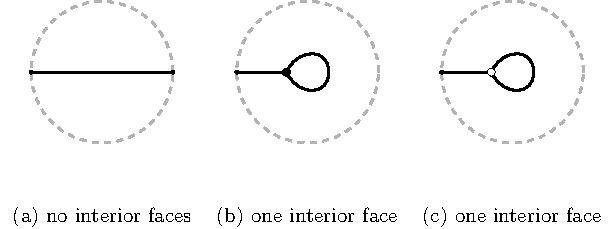
\includegraphics[width=0.6\textwidth]{../assets/840/trivred.pdf}
  \caption{\label{fig:trivred} Tail reductions that have boundary vertices.}
\end{figure}

\begin{proposition}\ \label{prop:simple_vs_moves}
\begin{itemize}
\item Suppose that two simple plabic graphs $G$ and $G'$ are move equivalent. Then $\QG$ and $\QX(G')$ are mutation equivalent.  
\item Any plabic graph $G'$ move equivalent to a simple plabic graph $G$ is also simple.
\end{itemize}
\end{proposition}
\begin{proof}
Direct check.
\end{proof}

%
%
%
%
%
%

%
%
%
%
%
%

\begin{figure}
  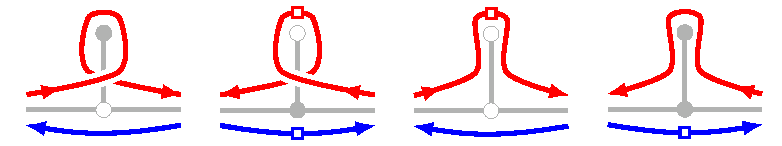
\includegraphics[width=0.65\textwidth]{../assets/840/interior_leaves.pdf}
  \caption{\label{fig:interior_leaves} The behavior of the link $\Lplab_G$ at interior leaves.}
\end{figure}

Recall from \cref{sec:intro:quivers-point-count} that each plabic graph gives rise to a link $\Lplab_G$ and that our main conjecture (\cref{conj:main}) yields a relation between the polynomials $\RQG(q)$ and $P(\Lplab_G;a,z)$.  For a rational function $R(q) = P(q)/Q(q)$, the \emph{leading coefficient} of $R(q)$ is defined as the ratio of the coefficient of $q^{\deg P}$ in $P(q)$ and the coefficient of $q^{\deg Q}$ in $Q(q)$. While \cref{conj:main} applies only to simple plabic graphs (cf. Section~9.3), the following more basic statement appears to hold for arbitrary plabic graphs.  In particular, we allow plabic graphs with interior leaves, though we still insist that interior faces are simply connected.  The link $\Lplab_G$ is defined as before, and the behavior of the strands at an interior leaf is shown in \cref{fig:interior_leaves}. 
 %
%
\begin{conjecture}\label{conj:top_a_deg}
Let $G$ be a plabic graph with $\conn(G)$ connected components and $n$ interior faces. Then the top $a$-degree of $P(\Lplab_G;a,z)$ equals
 \begin{equation}\label{eq:deg_a}
  %
  \degtop_a(P(\Lplab_G))=\conn(G)-n-1.
 \end{equation}
The degree of $\Ptop_L(q)$ (as a rational function in $q$) is given by
 \begin{equation}\label{eq:a_top}
\deg(\Ptop_L(q)) = n,
 \end{equation}
 and the leading coefficient of $\Ptop_L(q)$ is equal to $1$.
\end{conjecture}

Cluster varieties $\XQice$ are irreducible, with dimension equal to the number of vertices in $\Qice$.  Thus, when $R(Q;q)$ is a rational function, it has leading coefficient $1$ and degree equal to the number of vertices of $Q$.  So \cref{conj:main} implies \eqref{eq:a_top} for simple plabic graphs. %

%
%
%
%
%
%
%
%
%
%
%



%
%
%
%

\subsection{Empty quivers}
\begin{proposition}\label{prop:empty}
  Let $G$ be a connected plabic graph. The following are equivalent:
  \begin{enumerate}
  \item $\QG$ is empty.
  \item $G$ is a tree.
  \item\label{item:empty3} The tail reduction of $G$ is a graph with no interior vertices.
  \end{enumerate}
\end{proposition}
\begin{proof}
The mutable quiver $\QG$ is empty if and only if $G$ has no interior faces, which is equivalent to $G$ being a tree, since $G$ is assumed to be connected.  By Proposition~\ref{prop:trivred}, this is also equivalent to~\eqref{item:empty3}.
\end{proof}

\subsection{Disconnected graphs}
For two plabic graphs $G',G''$, we let $G'\disjun G''$ denote the disconnected plabic graph obtained by taking the disjoint union of $G'$ and $G''$. We denote by the same symbol the disjoint union of two quivers and of two links.
%
\begin{proposition}\label{prop:disc}
Suppose $G=G'\disjun G''$ is a disconnected plabic graph. Then $\QG=\QX(G')\disjun\QX(G'')$ and $\Lplab_G=\Lplab_{G'}\disjun \Lplab_{G''}$.
\end{proposition}
\begin{proof}
Follows directly from the definitions.
\end{proof}

\subsection{Isolated plabic graph quivers}
\newcommand\LHopf{L_{{\rm Hopf}}}
Recall that the \emph{connected sum} of two oriented knots $K, K'$ is defined as follows.  Find planar projections of the two knots that are disjoint.  Then find a (topological) rectangle $R$ in the plane, with oriented boundary consisting of sides $S_1,S_2,S_3,S_4$ in order, such that $S_1$ (resp. $S_3$) is an oriented arc along $K$ (resp. $K'$), and $S_2,S_4$ are disjoint from $K$ and $K'$.  The oriented connected sum knot $K \#K'$ is obtained by deleting $S_1,S_3$ and adding $S_2,S_4$.  To construct the connected sum of two links $L, L'$, we choose components $K \subset L$ and $K' \subset L'$ and perform the above surgery.  We call any link produced in this way the \emph{connected sum} of $L$ and $L'$, denoted $L \#L'$. The following result is well known; see e.g.~\cite[Proposition~16.2]{Lickorish}.

\begin{proposition}\label{prop:FLYsum}
Let $L$ and $L'$ be two oriented links.  Then $\HOMP(L \disjun L') = \left(\frac{a-a^{-1}}{z}\right)\HOMP(L)\HOMP(L')$ and $\HOMP(L \#L') = \HOMP(L) \HOMP(L')$. 
\end{proposition}
In particular, the $r$-component unlink has HOMFLY polynomial $\left(\frac{a-a^{-1}}{z}\right)^{r-1}$.

Let $\LHopf:=\hopflink$ denote the positively oriented Hopf link.  Then we have 
\begin{equation}\label{eq:Hopf}
\HOMP({\LHopf};a,z) = \frac{z + z^{-1}}{a} - \frac{z^{-1}}{a^{3}}.
\end{equation}



Recall that a quiver $Q$ is \emph{isolated} if it has no arrows.
\begin{proposition}\label{prop:plabic_isolated}
Let $G$ be a simple plabic graph with $n$ interior faces and $\conn(G)$ connected components. Suppose that $\QG$ is isolated. Then $\Lplab_G$ is a disjoint union of $\conn(G)$ links, each of which is a connected sum of some number (possibly zero) of positively oriented Hopf links. 
\end{proposition}
\begin{proof}
By Proposition~\ref{prop:disc}, we may assume that $G$ is connected.  Replace $G$ by its tail reduction (Proposition~\ref{prop:trivred}).
Then the result holds when $n = 0$: the link $\Lplab_G$ is an unknot.  The result also holds when $n =1$: the link $\Lplab_G$ is the Hopf link.  So suppose that $n > 1$.  In particular, we are assuming that $G$ has no boundary vertices.

\begin{figure}
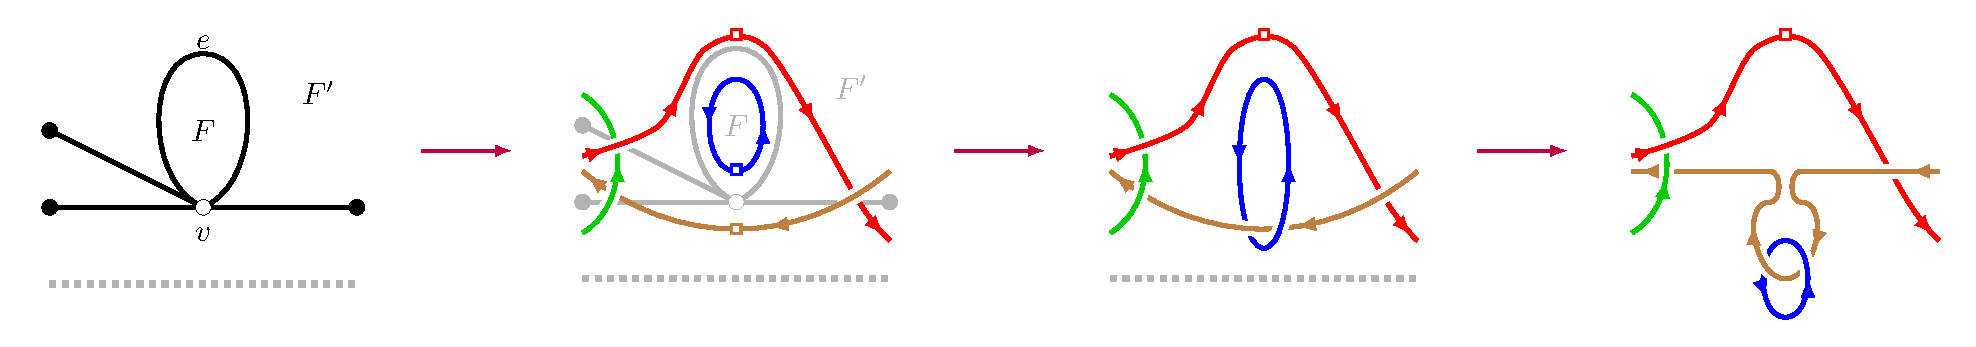
\includegraphics[width=1.0\textwidth]{../assets/840/loop_removal.pdf}
  \caption{\label{fig:loop_removal} A loop edge in $G$ whose sole vertex is adjacent to a boundary face results in having the Hopf link as a connected summand of $\Lplab_G$; see the proof of \cref{prop:plabic_isolated}.}
\end{figure}

For the remainder of the proof it is convenient to replace $G$ by its \emph{bipartite reduction}, obtained by contracting all interior edges whose endpoints have the same color. In particular, interior vertices are allowed to have degree higher than three.  Suppose first that $G$ contains an interior face $F$ which is bounded by a loop $e$ whose sole endpoint is $v\in V(G)$.  We show that $v$ must be adjacent to a boundary face of $G$. Without loss of generality, we may assume that the edge $e$ is not fully contained inside any other loop edge incident to $v$. Let $F'$ be the face on the other side of $e$ to $F$.  If $F'$ is a boundary face then we are done.  Otherwise, we assume that $F'$ is an interior face.  Let $e'$ be any non-loop edge incident to $v$ that is on the boundary of $F'$.  By our bipartite assumption, $e'$ connects $v$ to a vertex of opposite color.  The assumptions that $G$ is simple and $\QG$ is isolated then imply that $e'$ separates $F'$ from a boundary face.  It follows that $v$ is adjacent to a boundary face of $G$.  Letting $L':=\Lplab_{G-e}$, we see from \cref{fig:loop_removal} that $G$ is a connected sum of $L'$ and $\LHopf$. 
%
  Since $G-e$ has fewer interior faces, the result follows by induction.%

Suppose now that $G$, still assumed to be bipartite, has no interior faces that are bounded by loop edges. Let $F$ be an interior face of $G$. Since $G$ is simple, the perimeter of $F$ does not contain both sides of any edge. Moreover, since $\QG$ is isolated, every edge adjacent to $F$ is adjacent to a boundary face on the other side. Thus, $G$ consists of a number of interior faces connected in a tree-like manner as in \cref{fig:isolated_tree}.  The interior faces at the leaves of this tree must be bounded by loop edges, contradicting our assumption.
  %
\end{proof}

\begin{figure}
  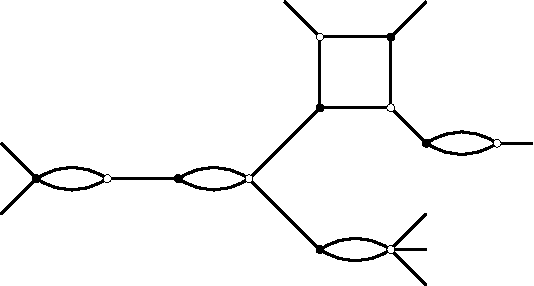
\includegraphics[width=0.4\textwidth]{../assets/840/isolatedtree.pdf}
  \caption{\label{fig:isolated_tree} A ``tree'' of interior faces (without boundary vertices) must have a loop.}
\end{figure}

\subsection{Torsion}
%
\newcommand\tF{\tilde F}
By definition, for $G$ a (possibly not simple) plabic graph, the quiver $\Qred_G$ is obtained from the directed graph $\QG$ (\cref{sec:intro:quivers-point-count}) by removing all $1$-cycles, and canceling out directed $2$-cycles one by one.  This agrees with the procedure in \cite{FPST}, and the mutation class of $\Qred_G$ is again invariant under the moves in \cref{fig:moves}. Note that $G$ is simple if and only if $\QG=\Qred_G$.

\begin{proposition}\label{prop:torsionfree}
Let $G$ be a plabic graph. Then $\QredG$ is torsion-free.
\end{proposition}
\begin{proof}
We prove the result by induction on the number of vertices of $\QredG$.  In the following, we index rows of the $\BQredG$ by interior faces $F$ of $G$.

We may suppose that $G$ is connected.  If $G$ has fewer than two interior faces, then checking the graphs in \cref{fig:trivred}, we see that the result holds.  So suppose that $G$ has at least two interior faces.  Applying tail removal, we may suppose that $G$ is not reduced.  Then by \cite{Pos}, one of the following holds: (a) $G$ has an interior leaf, or (b) the bipartite reduction (see the proof of \cref{prop:plabic_isolated}) has a loop, or (c) $G$ is move equivalent to a plabic graph with a two parallel edges between vertices of opposite color.

In case (a), removing the leaf vertex does not change $\QredG$.  We may thus assume that all interior leaves have been removed.  In case (b), deleting the loop edge removes a zero row and a zero column from $\BQredG$, so the result holds by induction.   We may thus assume that $G$ is leafless and loopless and we are in situation (c), that is, $G$ has a double edge: a pair $e',e''$ of edges between vertices $u,v$ of opposite colors.  Let $F$ be the interior face between $e'$ and $e''$, and let $F', F''$ be the faces on the other side of $e'$ and $e''$ to $F$; see \cref{fig:leafface}.   Let $G'$ be obtained from $G$ by removing both edges $e',e''$.  Let $B := \BQredG$, $C := B(\Qred_{G'})$, and $n := |V(\QredG)|$.  If $F',F''$ are both boundary faces, then $\Qred_{G'}$ is obtained from $\Qred_G$ by removing an isolated vertex, so the result holds by induction.  

Suppose that one of the faces $F',F''$ is boundary and one, say $F'$, is interior.    Then $\Qred_{G'}$ is obtained from $\Qred_G$ by removing the vertices $F$ and $F'$.  Let $\Z^V \cong \Z^n$ denote the free $\Z$-module with basis vectors $\{e_\E\}_{\E\in V}$ indexed by the vertex set $V = V(\Qred_G) = \{\mbox{interior faces $\E$ of $G$}\}$ and $\Z^{n-2} \cong \Z^{V'} \subset \Z^V$ the submodule spanned by basis elements other than $e_F, e_{F'}$.  The rows of $B$ belong to $\Z^V$ and the rows of $C$ belong to $\Z^{V'} \subset \Z^V$.  By induction, $C$ is torsion-free, so $\Z^{V'}/C^T \Z^{V'}$ has a basis given by some vectors $d_1,d_2,\ldots,d_r \in \Z^{V'}$.   Furthermore, we have
$$
b_F = \pm e_{F'}, \qquad b_{F'} \pm e_F \in \Z^{V'}, \qquad b_\E - c_\E \in  \Z e_{F'},  
$$
where $\E$ is any interior face other than $F,F'$, and $b_\E$ and $c_\E$ denote the rows of $B$ and $C$, respectively.  It is clear that $\Z^V/B^T \Z^V$ has a basis given by $\{d_1,\ldots,d_r\}$.  So $B$ is torsion-free.

Now suppose that $F',F''$ are both interior faces.  If $F' = F''$, then one of $u,v$, say $v$, must be a cut vertex of $G$.  Thus, $G$ contains a non-trivial induced subgraph $H$ containing $v$ and connected to $G-H$ only via $e',e''$.  The subgraph $H$ is contained ``inside" $F'=F''$; we may consider $H$ to be a plabic graph, necessarily not reduced, with a single boundary vertex incident to $v$.  Replacing $G$ by $H$ and repeating the argument, we are reduced the situation where $F' \neq F''$.

With $F' \neq F''$ both interior, $\Qred_{G'}$ is obtained from $\Qred_G$ by removing the vertex $F$ and identifying the vertices $F'$ and $F''$ to give a new vertex $\tF$ of $\Qred_{G'}$.  The rows of $B$ belong to $\Z^V \cong \Z^n$ and the rows of $C$ belong to $\Z^{V'} \cong \Z^{n-2}$, where $V' = V(\Qred_{G'})$.  Define the inclusion $\iota: \Z^{V'} \hookrightarrow \Z^V$ by sending $e_{\tF}$ to $e_{F'}$, and mapping the other basis vectors in the obvious way.  By induction, $C$ is torsion-free, so $\Z^{V'}/C^T\Z^{V'}$ has a basis given by some vectors $d_1,d_2,\ldots,d_r \in \Z^{V'}$.  We have that 
$$
b_F = \pm(e_{F'} - e_{F''}), \qquad b_{F'} +b_{F''} = \iota(c_{\tF}), \qquad b_\E - \iota(c_\E) \in \Z(e_{F'} - e_{F''}),
$$
where $\E$ is an interior face other than $F,F',F''$.  Let $W \subset \Z^{V - \{F\}}$ be the span of the vectors $b_F, b_{F'} +b_{F''}$ and $b_\E, \E \notin \{F,F',F''\}$.  Then $\{\iota(d_1),\ldots,\iota(d_r)\}$ form a basis of $\Z^{V- \{F\}}/W$.
But $b_{F'} \pm e_F \in\Z^{V - \{F\}}$, so $\Z^V/B^T\Z^V$ has basis $\{\iota(d_1),\ldots,\iota(d_r)\}$.  Thus, $B$ is torsion-free.
\end{proof}
Combining \cref{prop:torsionfree} with \cref{lem:ext}, we obtain the following result.
\begin{corollary}\label{cor:ext_simple}
Let $G$ be a simple plabic graph. Then $\QG$ admits a minimal extension.
\end{corollary}

\section{Skein relations}
In this section, we introduce leaf recurrent plabic graphs.  This class of plabic graphs includes the well-studied reduced plabic graphs and plabic fences.  We show that the leaf recurrence for plabic graphs corresponds to the skein relation for the associated links, thus establishing \cref{conj:main} for leaf recurrent plabic graphs.

\subsection{Leaf recurrent plabic graphs}\label{sec:leaf-recurr-plab}
In this section, we assume that all plabic graphs satisfy the assumptions of Section~\ref{sec:plabquiver}.

\begin{definition}
Let $G$ be a plabic graph. An interior face $F$ of $G$ is a \emph{boundary leaf face} if, in the tail reduction of $G$, the face $F$ has the form shown in \cref{fig:leafface}, i.e.  $F$ is bounded by two edges $e,e'$ with endpoints $u,v$ of distinct color, with $e$ separating $F$ from a boundary face and $e'$ separating $F$ from an interior face $F'$.
\end{definition}

\begin{figure}
  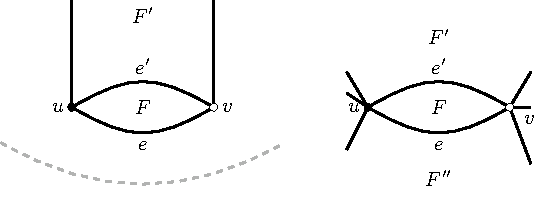
\includegraphics[width=0.7\textwidth]{../assets/840/leafface.pdf}
  \caption{\label{fig:leafface} A boundary leaf face $F$ (left) and an interior double edge (right).}
\end{figure}

\begin{lemma}\label{lemma:bdry_leaf_face}
Let $G$ be a simple plabic graph and $F$ a boundary leaf face. Let $u,v\in V(G)$ be the vertices adjacent to $F$. Then the plabic graphs $G':=G-e$ and $G'':=G-\{u,v\}$ are both simple.
\end{lemma}
\begin{proof}
The directed graph $\QX(G')$ is obtained from $\QG$ by removing the vertex corresponding to $F$.  Similarly, $\QX(G'')$ is obtained from $\QG$ by removing the vertices corresponding to $F$ and $F'$.  Both directed graphs are clearly quivers, and thus $G',G''$ are simple.
\end{proof}

\begin{definition}\label{dfn:leaf_recurrent_plabic_graph}
  The class of \emph{leaf recurrent} plabic graphs is defined as follows.
  \begin{enumerate}[(a)]%
  \item Every leaf recurrent plabic graph is simple.
  \item If $\QG$ is isolated then $G$ is leaf recurrent.
  \item If $G$ is move equivalent to a leaf recurrent plabic graph then $G$ is leaf recurrent.
  \item Suppose $G$ has a boundary leaf face $F$ as in \cref{lemma:bdry_leaf_face}. If the plabic graphs $G'$ and $G''$ are leaf recurrent then $G$ is leaf recurrent.
  \end{enumerate}
\end{definition}

\begin{remark}\label{rmk:leaf_rec=>Louise}
It is immediate that if $G$ is leaf recurrent then $\QG$ is \Louise.
\end{remark}

\begin{theorem}[{\cite[Remark~4.7]{MSLA}}]\label{thm:MSLA}
Any reduced plabic graph $G$ is leaf recurrent.
\end{theorem}



\subsection{The skein relation}\label{sec:sub_skein-relation}
%



\begin{figure}
  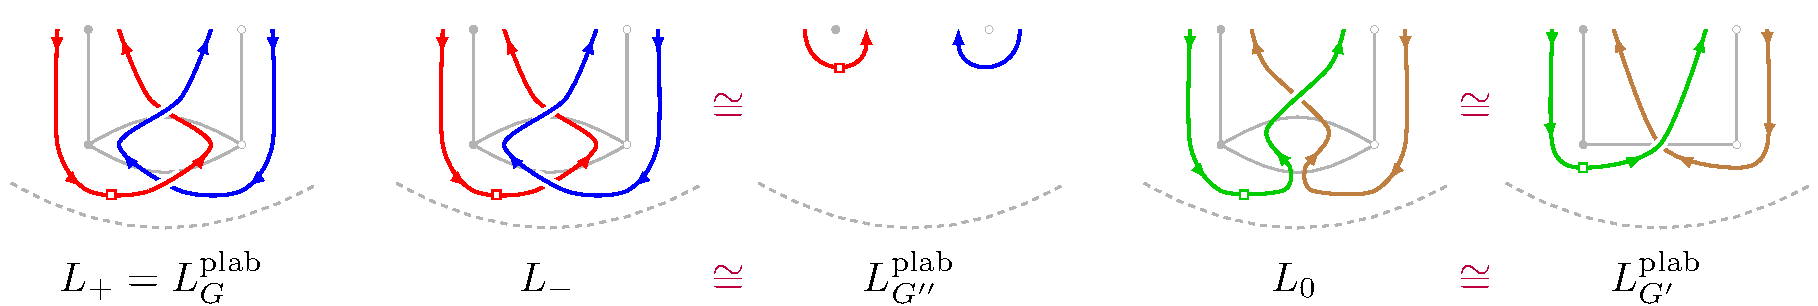
\includegraphics[width=1.0\textwidth]{../assets/840/skein.pdf}
  \caption{\label{fig:skein} Leaf recurrence for plabic graphs corresponds to the \FLY skein relation; see \cref{lemma:bdry_leaf_skein_FLY}.}
\end{figure}

\begin{lemma}\label{lemma:bdry_leaf_skein_FLY}
Suppose that $G$ is a plabic graph with a boundary leaf face $F$. Let $L_+:=\Lplab_G$, $L_0:=\Lplab_{G'}$, and $L_-:=\Lplab_{G''}$, where $G,G',G''$ are the three graphs in \cref{lemma:bdry_leaf_face}. Then the \FLY polynomials of $(L_+,L_0,L_-)$ are related by~\eqref{eq:HOMFLY_dfn}.
\end{lemma}
\begin{proof}
See \cref{fig:skein}.
\end{proof}

\begin{theorem}
  Suppose $G$ is a leaf recurrent plabic graph. Then Conjectures~\ref{conj:main} and~\ref{conj:top_a_deg} hold for $G$.
\end{theorem}
\begin{proof}
  Suppose $G$ has a boundary leaf face $F$ such that the graphs $G'$, $G''$ from \cref{lemma:bdry_leaf_face} are both leaf recurrent. Denote $Q:=\QG$, $Q':=\QX(G')$, $Q'':=\QX(G'')$, $L_+:=\Lplab_G$, $L_0:=\Lplab_{G'}$, and $L_-:=\Lplab_{G''}$, and note that $G,G',G''$ all have the same number of connected components.

By \cref{lemma:bdry_leaf_skein_FLY}, the \FLY polynomials of $(L_+,L_0,L_-)$ are related by~\eqref{eq:HOMFLY_dfn}. By \cref{rmk:leaf_rec=>Louise}, the quivers $Q,Q',Q''$ are \Louise. By \cref{cor:RQ_skein}, their point counts are related by~\eqref{eq:RQ_skein}. Comparing~\eqref{eq:HOMFLY_dfn} and~\eqref{eq:RQ_skein}, we see that~\eqref{eq:FLY=pcnt} holds for $Q$ if it holds for both $Q'$ and $Q''$.

Now suppose that $\QG$ is isolated with $n$ vertices.  If $G$ is the disjoint union of $G_1$ and $G_2$ then by Proposition~\ref{prop:FLYsum}, we have $\HOMP(\Lplab_{G})= ((a-a^{-1})/z)\HOMP(\Lplab_{G_1})\HOMP(\Lplab_{G_2})$, so $\Ptop_{\Lplab_G}(q) = (q-1)^{-1} \Ptop_{\Lplab_{G_1}}(q)\Ptop_{\Lplab_{G_2}}(q)$.  Since $\RQG(q) = \RQX{\QX(G_1)}{q}\RQX{\QX(G_2)}{q}$, the result follows. We may now assume that $G$ is connected.  By \cref{prop:plabic_isolated}, $\Lplab_G$ must be the connected sum of $n$ Hopf links.  By \cref{prop:FLYsum}, \eqref{eq:Hopf} and~\eqref{eq:A1} we have 
$$\Ptop_{\Lplab_G}(q) = \left(\frac{q^2-q+1}{q-1}\right)^n = \RQG(q).
$$
Thus, the result holds when $\QG$ is isolated.

Since the validity of~\eqref{eq:FLY=pcnt} is unchanged under moves on $G$, it follows that~\eqref{eq:FLY=pcnt} holds for all leaf recurrent plabic graphs $G$.  The equality~\eqref{eq:deg_a} also follows from the same argument.
\end{proof}

\subsection{Plabic fences}\label{sec:plabic-fences}
Following~\cite[Section~12]{FPST}, we consider the following class of plabic graphs. Let $\n\geq 2$ and let $I:=[\n-1]=\{1,2,\dots,\n-1\}$. A \emph{double braid word} is a word $\bw=(i_1,i_2,\dots,i_m)$ in the alphabet
\begin{equation*}%
  \pmn:=\{-1,-2,\dots,-(\n-1)\}\sqcup\{1,2,\dots,\n-1\}.
\end{equation*}
We denote the set of double braid words of length $m$ by $\DRW$. 

To a double braid word $\bw\in\DRW$ we associate a plabic graph $\Gbw$ with $2\n$ boundary vertices. First, draw $\n$ horizontal strands, with both endpoints of each strand on the boundary of the disk. Then for each $j=1,2,\dots,m$, let $h:=|i_j|$ and consider the strands at height $h$ and $h+1$. If $i_j>0$, add a black at $h$, white at $h+1$ bridge between these two strands, and if $i_j<0$, add a white at $h$, black at $h+1$ bridge between these two strands. The bridges are added one by one proceeding from left to right. See \cref{fig:PF2} for an example.

\begin{figure}
  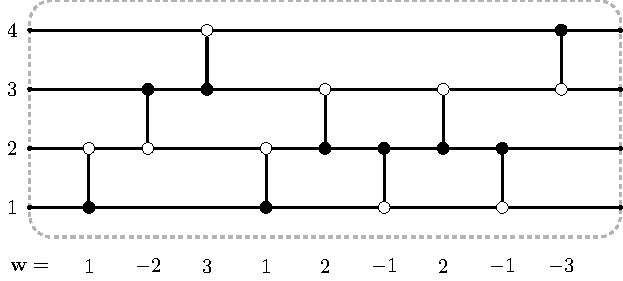
\includegraphics[width=0.7\textwidth]{../assets/840/plabic_fence-2.pdf}
  \caption{\label{fig:PF2} The plabic fence $\Gbw$ for a double braid word $\w$.}
\end{figure}

\begin{proposition}
For any $\bw\in\DRW$, the plabic graph $\Gbw$ is simple.
\end{proposition}
\begin{proof}
This is clear from construction. %
\end{proof}

Let us say that two braid words $\bw,\bw'$ are \emph{double braid move equivalent} if they are related by a sequence of the following moves:
\begin{enumerate}[(B1)]%
\item\label{bm1} $(\dots,i,j,i,\dots)\leftrightarrow (\dots,j,i,j,\dots)$ \quad if $i,j\in\pmn$ have the same sign and $|i-j|=1$;
\item\label{bm2} $(\dots,i,j,\dots)\leftrightarrow (\dots,j,i,\dots)$ \quad if $i,j\in \pmn$ have the same sign and $|i-j|>1$;
%
%
\item\label{bm5} $(\dots,i,j,\dots)\leftrightarrow (\dots,j,i,\dots)$  \quad if $i, j\in\pmn$ have different signs;
\item\label{bm6} $(-i,\dots)\leftrightarrow (i,\dots)$ \quad for $i\in \pmn$;
\item\label{bm7} $(\dots,-i)\leftrightarrow (\dots,i)$ \quad for $i\in \pmn$.
\end{enumerate}

%
%
%
%
%
It is clear that if $\bw,\bw'\in\DRW$ are double braid move equivalent then the plabic graphs $\Gbw,\GX(\bw')$ are  move equivalent.

\begin{proposition}
Plabic fences are leaf recurrent. That is, for any double braid word $\bw\in\DRW$, $\Gbw$ is a leaf recurrent plabic graph.
\end{proposition}
\begin{proof}
Proceed by induction on $m$. The base case $m=0$ is clear.

Applying moves~\ref{bm5}--\ref{bm6}, we may assume that $\bw$ has no negative indices. We say that a word $\bw=(i_1,i_2,\dots,i_m)\in I^m$ is \emph{reduced} if the associated permutation $\pi(\bw):=s_{i_1}s_{i_2}\cdots s_{i_m}$ has precisely $m$ inversions. If $\bw$ is not reduced then we may apply moves~\ref{bm1}--\ref{bm2} to transform $\bw$ into a word of the form $(\bw_1,i,i,\bw_2)$ for some $i\in I$ and some words $\bw_1\in I^{m_1}$, $\bw_2\in I^{m_2}$. Let $-\rev(\bw_1)\in (-I)^{m_1}$ denote the word obtained from $\bw_1$ by negating all indices and reversing their order. One can transform $\bw_1$ into $-\rev(\bw_1)$ by applying moves~\ref{bm5}--\ref{bm6}. Thus, applying moves~\ref{bm5}--\ref{bm6}, we transform
\begin{equation*}%
  (\bw_1,i,i,\bw_2)\to (-\rev(\bw_1),i,i,\bw_2)\to (i,i,\bw_2,-\rev(\bw_1)) \to (i,i,\bw_2,\bw_1).
\end{equation*}  The double bridge in $\GX(i,i,\bw_2,\bw_1)$ corresponding to $(i,i,\dots)$ gives rise to a boundary leaf face. Applying the induction hypothesis to the words $\bw':=(i,\bw_2,\bw_1)$ and $\bw'':=(\bw_2,\bw_1)$, we see that the plabic graphs $\GX(\bw')$ and $\GX(\bw'')$ are leaf recurrent. Thus, by \cref{dfn:leaf_recurrent_plabic_graph}, $\GX(\bw)$ is also a leaf recurrent plabic graph.

Finally, suppose that the word $\bw=(i_1,i_2,\dots,i_m)\in I^m$ is reduced. Then $\Gbw$ is a reduced plabic graph and therefore we are done by \cref{thm:MSLA}. Alternatively, applying moves~\ref{bm5}--\ref{bm6}, we may transform $\bw$ as follows:
\begin{equation*}%
  (i_1,i_2,\dots,i_m) \to (-i_1,i_2,\dots,i_m) \to (i_2,\dots,i_m,-i_1)\to (i_2,\dots,i_m,i_1).
\end{equation*}
We refer to this transformation as a \emph{conjugation move}. Applying conjugation and braid moves repeatedly, we either arrive at a non-reduced word and proceed by induction, or we find that $\pi(\bw)\in\Sn$ is a minimal length representative in its conjugacy class; see~\cite[Theorem~1.1]{GePf}. Recall that conjugacy classes in the symmetric group $\Sn$ correspond to cycle types, and $\pi(\bw)$ has minimal length  if and only if it is a product of cycles of the form $(a,a+1,\dots,b)$ on disjoint intervals $[a,b]\subset[\n]$. The resulting plabic fence $\Gbw$ has no interior faces and therefore is leaf recurrent.
\end{proof}
\begin{thebibliography}{MMMMMM}
\bibitem[1]{ACampo} A’Campo, Norbert Real deformations and complex topology of plane curve singularities, Ann. Fac. Sci. Toulouse Math. (6), Volume 8 (1999) no. 1, pp. 5-23 \href{https://alco.centre-mersenne.org/articles/10.5802/alco.345/#ACampo}{Publisher reference}.
\bibitem[2]{ALS} Arkani-Hamed, Nima; Lam, Thomas; Spradlin, Marcus Positive configuration space, Comm. Math. Phys., Volume 384 (2021) no. 2, pp. 909-954 \href{https://alco.centre-mersenne.org/articles/10.5802/alco.345/#ALS}{Publisher reference}.
\bibitem[3]{Arnold} Arnol’d, V. I. The geometry of spherical curves and quaternion algebra, Uspekhi Mat. Nauk, Volume 50 (1995) no. 1(301), pp. 3-68 \href{https://alco.centre-mersenne.org/articles/10.5802/alco.345/#Arnold}{Publisher reference}.
\bibitem[4]{BMS} Bazier-Matte, Véronique; Schiffler, Ralf Knot theory and cluster algebras, Adv. Math., Volume 408 (2022), Paper no. 108609, 45 pages \href{https://alco.centre-mersenne.org/articles/10.5802/alco.345/#BMS}{Publisher reference}.
\bibitem[5]{BHMPS} Blasiak, Jonah; Haiman, Mark; Morse, Jennifer; Pun, Anna; Seelinger, George H. A shuffle theorem for paths under any line, Forum Math. Pi, Volume 11 (2023), Paper no. e5, 38 pages \href{https://alco.centre-mersenne.org/articles/10.5802/alco.345/#BHMPS}{Publisher reference}.
\bibitem[6]{BuSc} Burban, Igor; Schiffmann, Olivier On the Hall algebra of an elliptic curve, I, Duke Math. J., Volume 161 (2012) no. 7, pp. 1171-1231 \href{https://alco.centre-mersenne.org/articles/10.5802/alco.345/#BuSc}{Publisher reference}.
\bibitem[7]{CG} Casals, Roger; Gao, Honghao Infinitely many Lagrangian fillings, Ann. of Math. (2), Volume 195 (2022) no. 1, pp. 207-249 \href{https://alco.centre-mersenne.org/articles/10.5802/alco.345/#CG}{Publisher reference}.
\bibitem[8]{CGGLSS} Casals, Roger; Gorsky, Eugene; Gorsky, Mikhail; Le, Ian; Shen, Linhui; Simental, José Cluster structures on braid varieties, 2022 \href{https://alco.centre-mersenne.org/articles/10.5802/alco.345/#CGGLSS}{Publisher reference}.
\bibitem[9]{CGGS} Casals, Roger; Gorsky, Eugene; Gorsky, Mikhail; Simental, José Positroid Links and Braid varieties, 2024 \href{https://alco.centre-mersenne.org/articles/10.5802/alco.345/#CGGS}{Publisher reference}.
\bibitem[10]{CW} Casals, Roger; Weng, Daping Microlocal theory of Legendrian links and cluster algebras, Geom. Topol., Volume 28 (2024) no. 2, pp. 901-1000 \href{https://alco.centre-mersenne.org/articles/10.5802/alco.345/#CW}{Publisher reference}.
\bibitem[11]{Deodhar} Deodhar, Vinay V. On some geometric aspects of Bruhat orderings. I. A finer decomposition of Bruhat cells, Invent. Math., Volume 79 (1985) no. 3, pp. 499-511 \href{https://alco.centre-mersenne.org/articles/10.5802/alco.345/#Deodhar}{Publisher reference}.
\bibitem[12]{FPST} Fomin, Sergey; Pylyavskyy, Pavlo; Shustin, Eugenii; Thurston, Dylan Morsifications and mutations, J. Lond. Math. Soc. (2), Volume 105 (2022) no. 4, pp. 2478-2554 \href{https://alco.centre-mersenne.org/articles/10.5802/alco.345/#FPST}{Publisher reference}.
\bibitem[13]{FWZ_book} Fomin, Sergey; Williams, Lauren; Zelevinsky, Andrei Introduction to Cluster Algebras. Chapters 1-3, 2021 \href{https://alco.centre-mersenne.org/articles/10.5802/alco.345/#FWZ_book}{Publisher reference}.
\bibitem[14]{FZ} Fomin, Sergey; Zelevinsky, Andrei Cluster algebras. I. Foundations, J. Amer. Math. Soc., Volume 15 (2002) no. 2, pp. 497-529 \href{https://alco.centre-mersenne.org/articles/10.5802/alco.345/#FZ}{Publisher reference}.
\bibitem[15]{HOMFLY} Freyd, P.; Yetter, D.; Hoste, J.; Lickorish, W. B. R.; Millett, K.; Ocneanu, A. A new polynomial invariant of knots and links, Bull. Amer. Math. Soc. (N.S.), Volume 12 (1985) no. 2, pp. 239-246 \href{https://alco.centre-mersenne.org/articles/10.5802/alco.345/#HOMFLY}{Publisher reference}.
\bibitem[16]{GL_cat_combin} Galashin, Pavel; Lam, Thomas Positroid Catalan numbers, 2021 \href{https://alco.centre-mersenne.org/articles/10.5802/alco.345/#GL_cat_combin}{Publisher reference}.
\bibitem[17]{GL_qtcat} Galashin, Pavel; Lam, Thomas Positroids, knots, and q,t-Catalan numbers, Sém. Lothar. Combin., Volume 85B (2021), Paper no. 54, 12 pages \href{https://alco.centre-mersenne.org/articles/10.5802/alco.345/#GL_qtcat}{Publisher reference}.
\bibitem[18]{GL_EHA} Galashin, Pavel; Lam, Thomas Monotone links in DAHA and EHA, 2023 \href{https://alco.centre-mersenne.org/articles/10.5802/alco.345/#GL_EHA}{Publisher reference}.
\bibitem[19]{GL_cluster} Galashin, Pavel; Lam, Thomas Positroid varieties and cluster algebras, Ann. Sci. Éc. Norm. Supér. (4), Volume 56 (2023) no. 3, pp. 859-884 \href{https://alco.centre-mersenne.org/articles/10.5802/alco.345/#GL_cluster}{Publisher reference}.
\bibitem[20]{GLSBS2} Galashin, Pavel; Lam, Thomas; Sherman-Bennett, Melissa Braid variety cluster structures, II: general type, 2023 \href{https://alco.centre-mersenne.org/articles/10.5802/alco.345/#GLSBS2}{Publisher reference}.
\bibitem[21]{GLSBS1} Galashin, Pavel; Lam, Thomas; Sherman-Bennett, Melissa; Speyer, David Braid variety cluster structures, I: 3D plabic graphs, 2022 \href{https://alco.centre-mersenne.org/articles/10.5802/alco.345/#GLSBS1}{Publisher reference}.
\bibitem[22]{GePf} Geck, Meinolf; Pfeiffer, Götz On the irreducible characters of Hecke algebras, Adv. Math., Volume 102 (1993) no. 1, pp. 79-94 \href{https://alco.centre-mersenne.org/articles/10.5802/alco.345/#GePf}{Publisher reference}.
\bibitem[23]{GN} Gorsky, Eugene; Neguţ, Andrei Refined knot invariants and Hilbert schemes, J. Math. Pures Appl. (9), Volume 104 (2015) no. 3, pp. 403-435 \href{https://alco.centre-mersenne.org/articles/10.5802/alco.345/#GN}{Publisher reference}.
\bibitem[24]{GNR} Gorsky, Eugene; Neguţ, Andrei; Rasmussen, Jacob Flag Hilbert schemes, colored projectors and Khovanov-Rozansky homology, Adv. Math., Volume 378 (2021), Paper no. 107542, 115 pages \href{https://alco.centre-mersenne.org/articles/10.5802/alco.345/#GNR}{Publisher reference}.
\bibitem[25]{HiIn} Hikami, Kazuhiro; Inoue, Rei Braids, complex volume and cluster algebras, Algebr. Geom. Topol., Volume 15 (2015) no. 4, pp. 2175-2194 \href{https://alco.centre-mersenne.org/articles/10.5802/alco.345/#HiIn}{Publisher reference}.
\bibitem[26]{Hirasawa} Hirasawa, Mikami Visualization of A’Campo’s fibered links and unknotting operation, Topology Appl., Volume 121 (2002) no. 1, pp. 287-304 \href{https://alco.centre-mersenne.org/articles/10.5802/alco.345/#Hirasawa}{Publisher reference}.
\bibitem[27]{KAT} The Knot Atlas: The Thistlethwaite Link Table \url{http://katlas.org/wiki/The_Thistlethwaite_Link_Table} \href{https://alco.centre-mersenne.org/articles/10.5802/alco.345/#KAT}{Publisher reference}.
\bibitem[28]{KAT_knot} The Knot Atlas: The Rolfsen Knot Table \url{http://katlas.org/wiki/The_Rolfsen_Knot_Table} \href{https://alco.centre-mersenne.org/articles/10.5802/alco.345/#KAT_knot}{Publisher reference}.
\bibitem[29]{KhoSoe} Khovanov, Mikhail Triply-graded link homology and Hochschild homology of Soergel bimodules, Internat. J. Math., Volume 18 (2007) no. 8, pp. 869-885 \href{https://alco.centre-mersenne.org/articles/10.5802/alco.345/#KhoSoe}{Publisher reference}.
\bibitem[30]{KR1} Khovanov, Mikhail; Rozansky, Lev Matrix factorizations and link homology, Fund. Math., Volume 199 (2008) no. 1, pp. 1-91 \href{https://alco.centre-mersenne.org/articles/10.5802/alco.345/#KR1}{Publisher reference}.
\bibitem[31]{KR2} Khovanov, Mikhail; Rozansky, Lev Matrix factorizations and link homology. II, Geom. Topol., Volume 12 (2008) no. 3, pp. 1387-1425 \href{https://alco.centre-mersenne.org/articles/10.5802/alco.345/#KR2}{Publisher reference}.
\bibitem[32]{KLS} Knutson, Allen; Lam, Thomas; Speyer, David E Positroid varieties: juggling and geometry, Compos. Math., Volume 149 (2013) no. 10, pp. 1710-1752 \href{https://alco.centre-mersenne.org/articles/10.5802/alco.345/#KLS}{Publisher reference}.
\bibitem[33]{LamCDM} Lam, Thomas Totally nonnegative Grassmannian and Grassmann polytopes, Current developments in mathematics 2014, Int. Press, Somerville, MA, 2016, pp. 51-152 \href{https://alco.centre-mersenne.org/articles/10.5802/alco.345/#LamCDM}{Publisher reference}.
\bibitem[34]{LS} Lam, Thomas; Speyer, David E Cohomology of cluster varieties I: Locally acyclic case, Algebra Number Theory, Volume 16 (2022) no. 1, pp. 179-230 \href{https://alco.centre-mersenne.org/articles/10.5802/alco.345/#LS}{Publisher reference}.
\bibitem[35]{LS2} Lam, Thomas; Speyer, David E Cohomology of cluster varieties II: Acyclic case, J. Lond. Math. Soc. (2), Volume 108 (2023) no. 6, pp. 2377-2414 \href{https://alco.centre-mersenne.org/articles/10.5802/alco.345/#LS2}{Publisher reference}.
\bibitem[36]{Lec} Leclerc, B. Cluster structures on strata of flag varieties, Adv. Math., Volume 300 (2016), pp. 190-228 \href{https://alco.centre-mersenne.org/articles/10.5802/alco.345/#Lec}{Publisher reference}.
\bibitem[37]{LeeSch} Lee, Kyungyong; Schiffler, Ralf Cluster algebras and Jones polynomials, Selecta Math. (N.S.), Volume 25 (2019) no. 4, Paper no. 58, 41 pages \href{https://alco.centre-mersenne.org/articles/10.5802/alco.345/#LeeSch}{Publisher reference}.
\bibitem[38]{Lickorish} Lickorish, W. B. Raymond An introduction to knot theory, Graduate Texts in Mathematics, 175, Springer-Verlag, New York, 1997, x+201 pages \href{https://alco.centre-mersenne.org/articles/10.5802/alco.345/#Lickorish}{Publisher reference}.
\bibitem[39]{knotinfo} Livingston, Charles; Moore, Allison H. KnotInfo: Table of Knot Invariants, 2022 \href{https://alco.centre-mersenne.org/articles/10.5802/alco.345/#knotinfo}{Publisher reference}.
\bibitem[40]{Mellit_Cell} Mellit, Anton Cell decompositions of character varieties, 2019 \href{https://alco.centre-mersenne.org/articles/10.5802/alco.345/#Mellit_Cell}{Publisher reference}.
\bibitem[41]{Muller} Muller, Greg Locally acyclic cluster algebras, Adv. Math., Volume 233 (2013), pp. 207-247 \href{https://alco.centre-mersenne.org/articles/10.5802/alco.345/#Muller}{Publisher reference}.
\bibitem[42]{Muller_skein} Muller, Greg Skein and cluster algebras of marked surfaces, Quantum Topol., Volume 7 (2016) no. 3, pp. 435-503 \href{https://alco.centre-mersenne.org/articles/10.5802/alco.345/#Muller_skein}{Publisher reference}.
\bibitem[43]{MSLA} Muller, Greg; Speyer, David E Cluster algebras of Grassmannians are locally acyclic, Proc. Amer. Math. Soc., Volume 144 (2016) no. 8, pp. 3267-3281 \href{https://alco.centre-mersenne.org/articles/10.5802/alco.345/#MSLA}{Publisher reference}.
\bibitem[44]{ObRo} Oblomkov, A.; Rozansky, L. Homfly-PT homology of Coxeter links, Transform. Groups, Volume 28 (2023) no. 3, pp. 1245-1275 \href{https://alco.centre-mersenne.org/articles/10.5802/alco.345/#ObRo}{Publisher reference}.
\bibitem[45]{OSS} Ozsváth, Peter S.; Stipsicz, András I.; Szabó, Zoltán Grid homology for knots and links, Mathematical Surveys and Monographs, 208, American Mathematical Society, Providence, RI, 2015, x+410 pages \href{https://alco.centre-mersenne.org/articles/10.5802/alco.345/#OSS}{Publisher reference}.
\bibitem[46]{Pos} Postnikov, Alexander Total positivity, Grassmannians, and networks (2006) \href{https://alco.centre-mersenne.org/articles/10.5802/alco.345/#Pos}{Publisher reference}.
\bibitem[47]{PT} Przytycki, Józef H.; Traczyk, Pawel Conway algebras and skein equivalence of links, Proc. Amer. Math. Soc., Volume 100 (1987) no. 4, pp. 744-748 \href{https://alco.centre-mersenne.org/articles/10.5802/alco.345/#PT}{Publisher reference}.
\bibitem[48]{Rolfsen} Rolfsen, Dale Knots and links, Mathematics Lecture Series, 7, Publish or Perish, Inc., Houston, TX, 1990, xiv+439 pages \href{https://alco.centre-mersenne.org/articles/10.5802/alco.345/#Rolfsen}{Publisher reference}.
\bibitem[49]{Ruth} Rutherford, Dan Thurston-Bennequin number, Kauffman polynomial, and ruling invariants of a Legendrian link: the Fuchs conjecture and beyond, Int. Math. Res. Not. (2006), Paper no. 78591, 15 pages \href{https://alco.centre-mersenne.org/articles/10.5802/alco.345/#Ruth}{Publisher reference}.
\bibitem[50]{ScVa} Schiffmann, Olivier; Vasserot, Eric The elliptic Hall algebra and the K-theory of the Hilbert scheme of 𝔸 2 , Duke Math. J., Volume 162 (2013) no. 2, pp. 279-366 \href{https://alco.centre-mersenne.org/articles/10.5802/alco.345/#ScVa}{Publisher reference}.
\bibitem[51]{Scott} Scott, J. S. Grassmannians and cluster algebras, Proc. London Math. Soc. (3), Volume 92 (2006) no. 2, pp. 345-380 \href{https://alco.centre-mersenne.org/articles/10.5802/alco.345/#Scott}{Publisher reference}.
\bibitem[52]{SSBW} Serhiyenko, K.; Sherman-Bennett, M.; Williams, L. Cluster structures in Schubert varieties in the Grassmannian, Proc. Lond. Math. Soc. (3), Volume 119 (2019) no. 6, pp. 1694-1744 \href{https://alco.centre-mersenne.org/articles/10.5802/alco.345/#SSBW}{Publisher reference}.
\bibitem[53]{SW} Shen, Linhui; Weng, Daping Cluster structures on double Bott-Samelson cells, Forum Math. Sigma, Volume 9 (2021), Paper no. e66, 89 pages \href{https://alco.centre-mersenne.org/articles/10.5802/alco.345/#SW}{Publisher reference}.
\bibitem[54]{STWZ} Shende, Vivek; Treumann, David; Williams, Harold; Zaslow, Eric Cluster varieties from Legendrian knots, Duke Math. J., Volume 168 (2019) no. 15, pp. 2801-2871 \href{https://alco.centre-mersenne.org/articles/10.5802/alco.345/#STWZ}{Publisher reference}.
\bibitem[55]{STZ} Shende, Vivek; Treumann, David; Zaslow, Eric Legendrian knots and constructible sheaves, Invent. Math., Volume 207 (2017) no. 3, pp. 1031-1133 \href{https://alco.centre-mersenne.org/articles/10.5802/alco.345/#STZ}{Publisher reference}.
\bibitem[56]{Trinh} Trinh, Minh-Tâm Quang From the Hecke Category to the Unipotent Locus, 2021 \href{https://alco.centre-mersenne.org/articles/10.5802/alco.345/#Trinh}{Publisher reference}.
\bibitem[57]{Turaev} Turaev, V. G. The Conway and Kauffman modules of a solid torus, Zap. Nauchn. Sem. Leningrad. Otdel. Mat. Inst. Steklov. (LOMI), Volume 167 (1988) no. 6, p. 79-89, 190 \href{https://alco.centre-mersenne.org/articles/10.5802/alco.345/#Turaev}{Publisher reference}.
\end{thebibliography}
\end{document}
